
\title{RECENT DEVELOPMENTS IN HODGE THEORY: A DISCUSSION OF TECHNIQUES AND RESULTS}
\markright{RECENT DEVELOPMENTS IN HODGE THEORY: A DISCUSSION OF TECHNIQUES AND RESULTS}

\author{By~ PHILLIP GRIFFITHS and WILFRIED SCHMID}
\markboth{PHILLIP GRIFFITHS and WILFRIED SCHMID}{RECENT DEVELOPMENTS IN HODGE THEORY: A DISCUSSION OF TECHNIQUES AND RESULTS}

\date{}
\maketitle

%\setcounter{page}{21}
\setcounter{pageoriginal}{20}


\section*{Introduction}\label{art4-sec1}
In\pageoriginale this paper, we shall review several recent developments in \textit{Hodge theory}, as applied to the study of the cohomology of algebraic varieties. In some sense, we are continuing the report \cite{art4-key21} of the first author, in which the then current work in Hodge theory was discussed without proof and a number of open problems were raised. Here we shall be concerned primarily with \textit{methods of proof}, \iec understanding in as transparent terms as possible the techniques utilized in this recent work in Hodge theory. We shall also present some results, due to the second author \cite{art4-key41}, which have just now been published, and shall bring up to date the status of the problems raised in \cite{art4-key21}.

One of the recent developments we shall discuss is Deligne's theory of \textit{mixed Hodge structures} (\cite{art4-key12}, \cite{art4-key}, \cite{art4-key14}). In this work, Deligne extends classical Hodge theory first to open, smooth varieties \cite{art4-key13}, then to complete, singular varieties \cite{art4-key14}, and finally to general varieties, also in \cite{art4-key14}. The heuristic reasoning explaining why such a theory should be possible is given in \cite{art4-key12}.

Deligne's technique is to use \textit{resolution of singularities} \cite{art4-key29}, in order to be able in each case to write the cohomology of the variety in question as being derived from the cohomology of K\"ahler manifolds by homological algebra. Typically this process gives the cohomology of the variety as the abutment of a spectral sequence whose $E_1$ or $E_2$ term is the cohomology of a smooth projective variety. Thus the $E_1$ or $E_2$ term has a \textit{Hodge structure}, and in order for this structure to survive as a Hodge structure on $E_\infty$, inducing the desired mixed Hodge structure on the cohomology of the variety, it is necessary that the spectral sequence degenerates. Following a discussion of the formalism of Hodge structures and mixed Hodge structures in \S 1, we have in \S 2 (a), \S 4, and \S 5 (d)  presented several typical degeneration arguments in as direct a manner as we could.

In \S \ref{art4-sec4} we construct the mixed Hodge structure on the cohomology of the simplest singular complete varieties, namely those having only \textit{normal crossings as singularities}. Here the main reason for the various degeneration theorems can be clearly isolated. The result in \S \ref{art4-sec4} stops far short of proving the existence of a mixed Hodge structure on the cohomology of a general singular variety \cite{art4-key14}. However, it is the method by which one most frequently \textit{calculates} this mixed Hodge structure (cf. \cite{art4-key10}, for instance), once it is known to exits.

In \S \ref{art4-sec5}, we have reproved the main result in the open case \cite{art4-key13} from a more analytic and less homological point of view. Our main idea is, instead of using the customary de Rham complex of $C^\infty$ forms on a compact K\"ahler manifold, to utilize a larger complex containing $L^1$-forms with certain precise types of singularities, and where the \textit{Gysin map} can be given on the form level preserving the Hodge filtration. This complex is discussed in \S\ref{art4-sec2}(b), where it is pointed out that the introduction of singular forms is necessary in order to have such a Gysin map on the form level. Operating inside this complex allows us to see clearly the differentials in the relevant spectral sequence in the open case, and to conclude the degeneracy result from the principle of two types (\S\S\ref{art4-sec5}(d), (e)).

Section 6 is devoted to some applications of Deligne's theory. First in \S \ref{art4-sec6}(a), we give his ``theorem on the fixed part'', which is the main tool in Deligne's study of the moduli of Hodge structures. Then, in \S\ref{art4-sec6}(b), we give a direct proof of an interesting result from \ref{art4-13}, concerning meromorphic differential forms on algebraic verieties; and finally we discuss an application of mixed Hodge structures to \textit{intermediate Jacobians} in \S \ref{art4-sec6}(c).

The second technique which we shall explore in some depth is the use of \textit{hyperbolic complex analysis}, as it applies to variation of Hodge structure. Hyperbolic complex analysis is the study of the influence of \textit{negative curvature} on holomorphic mappings. The classifying spaces for variation of Hodge structure are negatively curved, relative to the holomorphic maps which might arise in algebraic geometry (\cf \cite{art4-key11}, \cite{art4-key25}, and \S \ref{art4-sec3}(a), (b)), and so it is natural to apply the general philosophy in this case.

Following a discussion of the basic \textit{Ahlfors lemma} and its variants in \S \ref{art4-sec7}(a), we have given Borel's proof of the quasi-unipotence of the \textit{Picard-Lefschetz transformation} in \ref{art4-sec7}(b); this should illustrate in a simple fashion the power of the method.

Perhaps the most penetrating use of the philosophy of hyperbolic complex analysis occurs in the \textit{Nevanlinna theory} \cite{art4-key24}, which affords a general mechanism for analyzing the singularities of a holomorphic mapping. Following a preliminary result from Nevanlinna theory in \S \ref{art4-sec8}(a), we have used this technique to give rather simple, geometric proofs of \textit{Borel's extension theorem} \cite{art4-sec5} in \S \ref{art4-sec8}(b), and of the \textit{Riemann extension theorem for variation of Hodge structure} \cite{art4-key19} in \S \ref{art4-sec8}(c).

A final recent development we shall discuss is the work by the second author \cite{art4-key41} and joint work by him and Clemens \cite{art4-key10}, concerning the asymptotic behavior of the Hodge structures on the cohomology groups of an algebraic variety as it acquires singularities. In \S \ref{art4-sec9}(a), we have used the theorem on \textit{regular singular points} (\S \ref{art4-sec3} (c)), together with the Ahlfors lemma, to give an alternate proof of the first theorem from \cite{art4-sec41}. This result, the \textit{nilpotent} orbit theorem, reduces the case of a general degeneration of Hodge structure to the study of a special king a \textit{nilpotent orbit} in a classifying space for variation of Hodge structure. It seems possible to use Nevanlinna theory in place of the theorem on regular singular points to prove the same result, but we have not purshed this here.

The second main theorem from \cite{art4-key41}, the $SL_2$-\textit{orbit theorem}, gives a detailed and somewhat technical description of the nilpotent orbits which can come up when a one-parameter family of Hodge structures degenerates. The proof depends heavily on Lie theory. In \S \ref{art4-sec9}(b), besides stating the theorem, we describe the observations which originally led to the proof, as well as to the statement, of the theorem.

Some applications of these two theorems will be mentioned in \S\ref{art4-sec10}; we also summarize joint results of Clements and the second author about the topology of a degenerating family of projective manifolds, which again are partly based on the two theorems.

We conclude with an appendix, reviewing the current status of the problems and conjectures contained in the report \cite{art4-sec21} of the first author.

\section{Basic definitions}\label{art4-sec1}
(a)~ \textit{Hodge structures.} Let $H_{\bR}$ be a finite dimensional real vector space, containing a lattice $H_{\bZ}$, and let $H=H_{\bR} \otimes_{\bR} \bC$ be its complexification.

\begin{definition}\label{art4-def1.1}
`A Hodge structure of weight $m$' on $H$ consists of a direct sum decomposition
$$
H = \bigotimes_{p+q=m} H^{p,q}, \text{ with } H^{q,p} = \bar{H}^{p,q}
$$
\end{definition}

(Barring denotes complex conjugation.)

\begin{remark*}
The prototypical example is the decomposition according to Hodge type of the $m$-th complex cohomology group of a compact K\"ahler manifold. In this case, $m$, $p$, $q \;\geqslant 0$; however, it will be convenient to admit also negative values for $m$, $p$, and $q$. For example, the \textit{Hodge structure of Tate} $T$(1) is defined by
$$
H_{\bZ} =\bZ, \; H_{\bR} = \bR, \; H = \bC, \; m= -2, \text{ and } H = H^{-1,-1}.
$$

For any two Hodge structures $H, H'$, both of weight $m$, the direct sum $H\oplus H'$ carries an obvious Hodge structure, also of weight $m$. Similarly, if $H$ and $H'$ have possibly different weight $m$ and $m'$,
$$
H\otimes H', \; \Hom (H, H'), \Lambda^p H, \; H^\ast
$$
inherit Hodge structures of weight $m+ m'$, $m'-m$, $pm$, and $-m$, respectively: $\lambda \in \Hom(H, H')$ has Hodge type $(p,q)$ if $\lambda(H^{r,s}) \subset (H')^{p+r, \; q+s}$ for all $r, s$; in particular, this definition applies to $H^\ast = \Hom (H, \bC)$, with $\bC$ carrying the trivial Hodge structure of weight $0; H \otimes H'$ can be identified with $\Hom (H^\ast, H')$, and $\otimes^pH$ induces a Hodge structure on its subspace $\Lambda^p H$.
 \end{remark*}

\begin{definition}\label{art4-def1.2}
A linear map $\varphi: H \to H'$ between vector spaces with Hodge structures will be called a morphism (of Hodge structures) if it is defined over $\bQ$, relative to the lattices $H_{\bZ}$, $H'_{\bZ}$, and if $\varphi (H^{p,q}) \subset (H')^{p,q}$, for all $p,q$. More generally, $\varphi$ is a morphism of type $(r,r)$ if again it is defined over $\bQ$, and if it has type ($r, r$) when viewed as an element of $\Hom(H, H')$.
\end{definition}

As a trivial, but nevertheless important, observation we note that morphism of type $(r,r)$ must vanish unless the weights $m$ and $m'$ of $H$ and $H'$ satisfy $m'=m+2r$.

To\pageoriginale each Hodge structure $H = \oplus_{p+q =m} H^{p,q}$ of weight $m$ one associates the \textit{Hodge filtration}
\setcounter{equation}{2}
\begin{equation}
H \supset \ldots \subset F^{p-1} \supset F^p \subset F^{p+1} \supset \ldots \supset 0 \text{ with } F^p = \oplus_{i \geqslant p} H^{i, m-i}.  \label{art4-eq1.3}
\end{equation}

It may be convenient to visualize the definition by means of the picture below:
\begin{figure}[H]
\centering
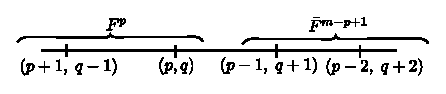
\includegraphics{art4-fig1.eps}
\end{figure}

The Hodge filtration determines the Hodge structure completely, since
\begin{equation}
H^{p,q} = F^p \cap \bar{F}^q \label{art4-eq1.4}
\end{equation}

Conversely, a descending filtration $\{F^p\}$ of $H$ arises as the Hodge filtration of some Hodge structure of weight $m$ if and only if
\begin{equation}
F^p \oplus \bar{F}^{m-p+1} \xrightarrow{\approx} H, \;\; \text{ for all } p.
\label{art4-eq1.5}
\end{equation}

Thus one has a 1:1 correspondence between Hodge structures and Hodge filtrations, \iec filtrations satisfying \eqref{art4-eq1.5}.

In terms of this latter description, a linear map $\varphi: H \to H'$, which shall be defined over $\bQ$, becomes a morphism of type $(r, r)$ exactly when it preserves the Hodge filtration, with a shift by $r$; in other words, when 
\begin{equation}
\varphi (F^p) \subset F'^{p+r}, \;\text{ for all }p. \label{art4-eq1.6}
\end{equation}

Now let $\varphi$ be a morphism of type $(r, r)$, $v$ a vector in $F'^{p+r} \cap \Iim \varphi$. By decomposing a vector in the inverse image of $v$ according to Hodge type, one finds that $v$ lies in the image of $F^p$. Thus:

a morphism of Hodge structures of type $(r,r)$ preserves the Hodge filtrations strictly, with a shift by $r$, in the sense that 
\begin{equation}
\varphi(F^p) = F'^{p+r} \cap \Iim \varphi, \text{ for all } p. 
\label{art4-eq1.7}
\end{equation}

We consider a Hodge structure $H = \oplus_{p+q = m} H^{p,q}$ and a bilinear form $Q$ on $H$, which shall be defined over $\bQ$. Also $Q$ shall be symmetric if $m$ is even, skew if $m$ is odd.

\setcounter{definition}{7}
\begin{definition}\label{art4-def1.8}
The Hodge structure is polarized by $Q$ if 
$$
\begin{matrix}
Q (H^{p,q} , H^{p', q'} =0) & \text{ unless } p = q', \; q = p',\\[2pt]
(\sqrt{-1})^{p-q} Q (v, \bar{v}) > 0 & \text{ for } v \in H^{p,q}, \; v \neq 0.
\end{matrix}
$$
\end{definition}

Apparently, the polarization form $Q$ must be nondegenerate. The Weil operator $C: H \to H$ of the Hodge structure is defined by 
\setcounter{equation}{8}
\begin{equation}
C_v = (\sqrt{-1})^{p-q} v, \text{ for } v \in H^{p,q} . \label{art4-eq1.9}
\end{equation}
In terms of the Hodge filtration and the Weil operator, the two conditions in \ref{art4-def1.8} become equivalent to 
\begin{equation}
\left.
\begin{matrix}
Q (F^p, F^{m-p+1}) = 0\\
Q (C v, \bar{v}) >0 \;\text{  for } v \neq 0.
\end{matrix}\right\}
\label{art4-eq1.10}
\end{equation}

The example we have in mind is the Hodge bilinear form on the primitive part of the cohomology of a smooth, projective variety over $\bC$, as will be discussed below.

It should be mentioned that the operations of tensor product, Hom exterior product, and duality can also be performed in the context of polarized Hodge structures. For example, if $Q$ and $Q'$ are polarization forms for Hodge structures $H$ and $H'$, then the induced bilinear form on $H \otimes H'$ polarizes the product Hodge structure.

\medskip
\noindent
(b)~ \textit{Mixed Hodge structures.} The symbols $H$, $H_{\bR}$, $H_{\bZ}$ shall have the same meaning as in the previous section.

\begin{definition}\label{art4-def1.11}
`A mixed Hodge structure' on $H$ consists of two filtrations,
$$
0 \subset \ldots \subset W_{m-1} \subset W_m \subset W_{m+1} \subset \ldots \subset H,
$$
the `weight filtration' which shall be defined over $\bQ$, and 
$$
H \supset \ldots \supset F^{p-1} \supset F^p \supset F^{p+1} \supset \ldots \supset 0,
$$
the `Hodge filtration', such that the filtration induced by the latter on $Gr_m(W_\ast) = W_m/W_{m-1}$ defines a Hodge structure of weight $m$, for each $m$ (the induced filtration on $Gr_m(W_\ast)$ is given by
$$
F^p (Gr_m (W_\ast)) = W_m \cap F^p/W_{m-1} \cap F^p).
$$
\end{definition}


\begin{remark*}
The notion\pageoriginale of a mixed Hodge structure contains that of a Hodge structure of weight $m$ as a special case; as Hodge filtration one takes the Hodge filtration in the old sense, and the weight filtration is defined by $W_m = H$, $W_{m-1} = 0$.
\end{remark*}

According to the definition of a mixed Hodge structure, only the successive quotients of the weight filtration have direct sum decompositions according to Hodge type. However, the following lemma of Deligne \cite{art4-key13} provides a more subtle global decomposition of $H$. For any pair of integers $(p,q)$, we consider the subspace
\begin{multline*}
I^{p,q} = (F^p \cap W_{p+q}) \cap (\bar{F}^q \cap W_{p+q} + \bar{F}^{q-1} \cap W_{p+q-2} +\\
 + \bar{F}^{q-2} \cap W_{p+q-3} + \ldots).
\end{multline*}
It is certainly not the case that $I^{p,q} = I^{q,p}$, but one does have the congruence $I^{p,q} \equiv I^{q,p} \mod W_{p+q-2}$, as will follow from the proof of lemma \ref{art4-lem1.12} below. This congruence $I^{p,q} \equiv \bar{I^{q,p}} \mod  W_{p+q-2}$ explains why every mixed Hodge structure with a weight filtration of length two splits over $\bR$, into a sum of two Hodge structures of pure weight. This splitting, of course, may be incompatible with the rational structure. As soon as the weight filtration has length greater than two, a ``general'' mixed Hodge structure will not split over $\bR$.

\setcounter{lemma}{11}
\begin{lemma}[\cf Lemma 1.2.8 of \cite{art4-key13}.]\label{art4-lem1.12}
Under the projection $W_m \to Gr_m (W_\ast), \; I^{p,q}$, with $p+q=m$, maps isomorphically onto the Hodge subspace $Gr_m (W_\ast)^{p,q}$. Moreover,
$$
W_m = \oplus_{p+q\leqslant m} I^{p,q},
$$
and 
$$
F^p = \oplus_{i \geqslant p} \oplus_q I^{p,q}.
$$
\end{lemma}

\begin{proof}
In view of \eqref{art4-eq1.5}, the definition of a mixed Hodge structure amounts to the following:
\begin{align*}
& \text{given any $v \in W_n$ and integers $p,q$, with $p+q=m+1$,}\\
& \text{one can write $v = v'+\bar{v}'' + u $, such that $v' \in F^p \cap W_m$,}\\
& \text{$v'' \in F^q \cap W_m$, and $u\in W_{m-1}$; this decomposition is unique}\\
& \text{modulo $W_{m-1}$}. \tag{$\ast$}\label{art4-eq*}
\end{align*}

In order to prove the first assertion of the lemma, we fix $m$, $p$, $q$, subject to $m=p+q$, and $\alpha \in Gr_m (W_\ast)^{p,q}$. Then $\alpha$ can be represented by some\pageoriginale $v_0\in F^p \cap W_m$, and also by some $\bar{u}_0 \in \bar{F}^q \cap W_m$. Both are unique upto $W_{m-1}$, and $v_0 = \bar{u}_0 + w_0$, for some $w_0 \in W_{m-1}$. By induction on $k$, starting with $k=0$, we shall find vectors
\begin{gather*}
v_k \in F^p \cap W_m, \qquad w_k \in W_{m-1-k}\\
u_k \in F^q \cap W_m + F^{q-1} \cap W_{m-2} + F^{q-2} \cap W_{m-3} + \ldots + F^{q+1-k} \cap W_{m-k}
\end{gather*}
which will be unique up to $W_{m-k}$, such that $v_k$ represents $\alpha$, and $v_k = \bar{u}_k + w_k$. For $k=0$, this has been done $(F^{q+1} \subset F^q !)$.  If $v_k$, $u_k$, $w_k$ have been picked, we apply \eqref{art4-eq*} to $w_k$: we write $w_k = w'_k + \bar{w}''_k + w_{k+1}$, with $w'_k \in F^p \cap W_{m-1-k}$, $w_k \in F^{p-k} \cap W_{m-1-k}$, $w_{k+1} \in W_{m-2-k}$, uniquely modulo $W_{m-2-k}$. The vectors $w_{k+1}, \; v_{k+1} = v_k - w'_k$, $u_{k+1} =  u_k + w''_k$ then have the desired properties. For large enough $k$, $W_{m-1-k} = 0$; hence $\alpha$ has a unique representative in $I^{p,q}$. We may deduce that
$$
W_m = W_{m-1} \oplus (\oplus_{p+q=m} I^{p,q}),
$$
and thus $W_m = \oplus_{p+q\leqslant m} I^{p,q}$. As for the last statement of the lemma, the sum of the $I^{p,q}$ is now known to be direct. Also, one containment is obvious. We consider some $v \in F^p$, and we let $m$ be the least integer for which $v \in W_m$. The image of $v$ in $Gr_m (W_\ast)$ has Hodge components of type $(i, m-i)$, with $i \geqslant p$, because $v \in F^p \cap W_m$. Subtraction off components in the spaces $I^{i,m-i}$, with $i \geqslant p$, we can push $v$ into $W_{m-1}$. Continuing with descending induction on $m$, we find that $v \in \oplus_{i \geqslant p} \oplus \oplus_q I^{i,q}$, as was to be shown.
 
A \textit{morphism} between two mixed Hodge structures $\{H, W_m, F^p\}$,\break $\{H', W'_m, F'^p\}$ is a rationally defined linear $\map \varphi; H \to H'$, such that $\varphi(W_m) \subset W'_m$ and $\varphi (F^p) \subset F'^p$. More generally, a rationally defined linear $map \varphi : H \to H'$ will be called a morphism of mixed Hodge structures of type $(r,r)$ if $\varphi (W_m) \subset W'_{m+2r}$, $\varphi (F^p) \subset F'^{p+r}$, for all $p$ and $m$. In this case, the induced mapping
$$
\varphi: Gr_m (W_\ast) \to Gr_{m+2r} (W'_\ast)
$$
becomes a morphism of type $(r,r)$ relative to the two Hodge structures of weights $m$ and $m+ 2r$, respectively.
\end{proof}

\setcounter{lemma}{12}
\begin{lemma}\label{art4-lem1.13}
A morphism\pageoriginale of type $(r,r)$ between mixed Hodge structures is strict with respect to both the weight and Hodge filtrations, with the appropriate shift in indices. More precisely, $\varphi (W_m) = W'_{m+2r} \cap \Iim \varphi, \; \varphi (F^p) = F'^{p+r} \cap \Iim \varphi$.
\end{lemma}

\begin{proof}
The definition of the subspaces $I^{p,q}$ immediately gives the containments $\varphi(I^{p,q}) \subset I'^{p+r, q+r}$. Now let $v \in W'_{m+2r} \cap \Iim \varphi$, so that $v = \varphi (u)$ for some $u \in H$. According to \ref{art4-lem1.12},
$$
u = \sum_{p,q} u^{p,q}, \text{ with } u^{p,q} \in I^{p,q}.
$$
Then $\varphi (u^{p,q}) \in I'^{p+r , q+r}$, and $v =\sum_{p,q} \varphi (u^{p,q}) =in W'_{m+2r}$. Again appealing to \ref{art4-lem1.12}, we deduce that $\varphi(u^{p,q}) =0$, unless $p+q \leqslant m$. Hence
$$
v = \varphi \left(\sum_{p+q \leq m} u^{p,q} \right) \in \varphi (W_m).
$$

The case of the Hodge filtration is treated similarly.
\end{proof}

\begin{lemma}\label{art4-lem1.14}
Let $\varphi: H \to H'$ be a morphism of mixed Hodge structures of type $(r,r)$. Then the induced Hodge and weight filtrations put mixed Hodge structure both on the kernel and the cokernel.
\end{lemma}

\begin{proof}
As for the kernel, given $v \in \ker \varphi \cap W_m$ and any integer $p$, we must exhibit vectors
$$
v'\in \ker \varphi \cap W_m \cap F^p, \; v'' \in \ker \varphi \cap W_m \cap F^{m-p+1}, \; w \in \ker \varphi \cap W_{m-1},
$$
such that $v = v' + \bar{v}''+u$, and these must be uniquely determined modulo $\ker \varphi \cap W_{m-1}$. The uniqueness already follows from the corresponding statement about $H$. Also, there do exist $u'\in W_m \cap F^p$, $u'' \in W_m \cap F^{n-p+1}$, such that $v \equiv u' + \bar{u}'' \mod W_{m-1}$. Since $\varphi(v) = 0$, we conclude that $\varphi (u')$, $\varphi (u'') \in W'_{m+2r-1}$. By appealing to \ref{art4-lem1.12} and decomposing $u'$ into its components in the subspaces $I^{s,t} \subset H$, we can find $u'_1 \in W_{m-1} \cap F^p$, so that  $\varphi(u') = \varphi(u'_1)$. Similarly, $\varphi (u'') = \varphi (u''_1)$ for some $u''_1 \in W_{m-1} \cap F^{m-p+1}$. The vectors $v'= u'-u'_1$, $v''=u'' - u''_1$, $w = v - v'-\bar{v}''$ have the desired properties. In order to prove the assertion about the cokernel, one only has to check one nontrivial fact: if $u \in W'_m \cap F'^p$, $v \in W'_m \cap F'^{m-p+1}$, and if $u + \bar{v} \in w'_{m-1} +\Iim \varphi$, then $u, v\in W'_{m-1} + \Iim \varphi$. Using \ref{art4-lem1.12}, this can be done, in a manner similar to the argument above. Details are left to the reader.
\end{proof}

\setcounter{coro}{14}
\begin{coro}\label{art4-coro1.15}
Let $(H^\ast, d)$ be a finite dimensional complex with a mixed Hodge structure, and such that the differential $d$ is a morphism of mixed Hodge structures of type $(r,r)$, for some $r$. Then in induced filtrations on the cohomology determine a mixed Hodge structure.
\end{coro}

As a final remark, whose verification is left to the reader, we want to add the 

\setcounter{observation}{15}
\begin{observation}\label{art4-obser1.16}
Let $0 \to H' \to H \to H'' \to 0$ be an exact sequence of vector spaces. If two filtrations $\{W_l\}$ and $\{F^p\}$ for $H$ induce mixed Hodge structures on both $H'$ and $H''$, then they determine a mixed Hodge structure on $H$ itself.
\end{observation}

\section{Classical Hodge theory}\label{art4-sec2}
(a)~ \textit{The cohomology of a K\"ahler manifold}. Let $V$ be a compact, complex manifold of dimension $n$, and $A^\ast (V)$ the de Rham complex of $C^\infty$ forms on $v$. The decomposition into type
$$
A^\ast (V) = \oplus_{p,q} A^{p,q} (V)
$$
reflects the complex structure on $V$, and \textit{via} de Rham's theorem has implications in the cohomology $H^\ast (V, \bC)$. However, not very much is known about this unless $V$ is K\"ahler, or at least nearly K\"ahler. In this case, there are two main sources for the many profound implications which the complex structure plus the K\"ahler metric have in the coholomogy, and we shall briefly discuss these.

Suppose that $ds^2_V = \Sigma_{i,j} g_{ij} dz_i dz_j$ is a K\"ahler metric with fundamental (1,1)-form $\omega = \dfrac{\sqrt{-1}}{2} \Sigma_{i,j} g_{ij} dz_i \wedge d\bar{z}_j$. The operators 
\begin{align*}
& L: A^k (V) \to A^{k+2} (V)\\ 
& \wedge : A^k (V) \to A^{k-2} (V)
\end{align*} 
are defined by $L (\varphi) = \omega \wedge \varphi$ and $\Lambda =$  adjoint of $L = \pm \ast L\ast$, where $\ast : A^k (V) \to A^{2n-k} (V)$ is the duality or ``star'' operator. 

Letting 
$$
P: A^k (V) \to A^k (V)
$$
be given\pageoriginale  by $P(\varphi) = (k-n)\; \varphi$, the commutation relations
\setcounter{equation}{0}
\begin{equation}
\left.
\begin{matrix}
[L, \Lambda]  = P\\
[P, L]  = 2L\\
[P, \Lambda]  = - 2 \Lambda 
\end{matrix}
\right] \label{art4-eq2.1}
\end{equation}
exactly say that we have a Lie algebra homomorphism
$$
\rho: \fs\fl(2) \to \End (A^\ast (V)),
$$
given by 
\begin{align*}
\rho (E_+) & = L \\
\rho(E_-) & = \Lambda\\
\rho (H) & = P,
\end{align*}
where $E_+ = \left(\begin{smallmatrix}
0 & 1\\
0 & 0
\end{smallmatrix} \right)$, $E_- = \left(\begin{smallmatrix}
0 & 0\\
1 & 0
\end{smallmatrix} \right)$, and $H = \left(\begin{smallmatrix}
1 & 0\\
0 & -1
\end{smallmatrix} \right)$ are the usual basis elements for $\fs \fl$ (2). The first main source for the structure on $H^\ast(V)$ arises from the commutation relation
\begin{equation}
[\rho, \Delta] = 0 \label{art4-eq2.2}
\end{equation}
where $\Delta = dd^\ast + d^\ast d$ is the Laplacian associated to $ds^2_v$.\footnote{Here we are adopting the viewpoint of Chern \cite{art4-key7} (see also \cite{art4-key46}), where the proofs of our statements can be found. Alternate sources are \cite{art4-key45} or \cite{art-4key47}.} Letting $\sH^\ast(V) =\{\varphi \in A^{\ast} (V) : \Delta \varphi = 0\}$ be the \textit{harmonic forms} the \textit{Hodge theorem} \cite{art4-key44}.
$$
\sH^\ast (V) \xrightarrow{\approx} H^\ast_{DR} (V)
$$
together with \eqref{art4-eq2.2} tells us that $\rho$ induces a representation
\begin{equation}
\rho_\ast : \fs\fl (2) \to \End (H^\ast (V)) \label{art4-eq2.4}
\end{equation}
on the cohomology level. Applying the standard facts about representations of $\fs \fl$ to $\rho_\ast$, one obtains first the so-called \textit{Hard Lefschetz theorem}
\begin{equation}
L^k : H^{n-k} (V) \xrightarrow{\approx} H^{n+k} (V), \label{art4-eq2.4}
\end{equation}
and secondly the \textit{Lefschetz decomposition}
\begin{equation}
H^l (V) = \oplus_{0 \leqslant k \leqslant [l/2]} L^k p^{l-2k} (V), \label{art4-eq2.5}
\end{equation}\pageoriginale
where 
\begin{equation}
p^{n-k} (V) = \ker\{H^{n-k} (V) \xrightarrow{L^{k+1}} H^{n+k+2} (V)\} \label{art4-eq2.6}
\end{equation}
is the \textit{primitive part} of $(n-k)$th cohomology group.

We shall briefly discuss an application of \eqref{art4-eq2.4} and \eqref{art4-eq2.5} to prove degeneration of a spectral sequence; the argument it due to Blanchard and Deligne.

Let $X$ be a K\"{a}hler manifold (possibly non-compact), $S$ a complex manifold, and 
$$
f: X \to S
$$
a smooth, proper holomorphic mapping.\footnote{$f: X \to S$ is a differential fibre bundle whose fibres are compact K\"{a}hler manifolds; \cf \S \ref{art4-sec3} for further discussion.} The \textit{Theorem of Leray} \cite{art4-key17} gives a spectral sequence $\{E_r\}$ with 
\begin{gather*}
E^{p,q}_2 = H^p (S, R^q_{f_\ast} (\bC))\\
E_{\infty} \Rightarrow H^\ast (X)
\end{gather*}
where the \textit{direct image sheaf} $R^\ast_{f_\ast} (\bC)$ comes from the presheaf
$$
U \to H^\ast (f^{-1} (U), \bC).
$$
The theorem asserts that $E_2 = E_\infty$.

To prove this, we remark that the K\"{a}hler metric on $X$ induces operators $L$, $\Lambda$ on the direct image sheaves $R^\ast_{f_\ast} (\bC)$ which commute with the differentials in the spectral sequence. In particular, the hard Lefschetz Theorem \eqref{art4-eq2.4} and Lefschetz decomposition \eqref(art4-eq2.5) become
\begin{gather*}
L^k : R^{n-k}_{f_\ast} (\bC) \xrightarrow{\approx} R^{n+l}_{f_\ast} (\bC)\\
R^l_{f_{\ast}} (\bC) = \oplus_k L^k P^{l-2k}_{f_\ast} (\bC),
\end{gather*}
where $P^{l-2k}_{f_\ast} = \ker \{L^{k+1}: R^{n-k}_{f_\ast} (\bC) \to R^{n+k+2}_{f_\ast}\}$. We shall check that $d_2 =0$, the proof that the higher $d_r=0$ being the same. Using the Lefschetz decomposition, it will suffice to show that $d_z =0$ on $P^{n-k}_{f_\ast} (\bC)$. Now in the diagram
$$
\xymatrix{
H^p (S, P^{n-k}_{f_\ast} (\bC)) \ar[d]^{d_2} \ar[r]^{L^{k+1}} & H^p (S, R^{n+k+2}_{f_\ast} (\bC)) \ar[d]^{d_2}\\
H^{p+2} (S, R^{n-k-1}_{f_\ast} (\bC))  \ar@{^{(}->}[r]^{L^{k+1}} & H^{p+2} (S, R^{n+k+1}_{f_\ast} (\bC)),
}
$$
the bottom row is injective by Hard Lefschetz and the top row is zero by the definition of primitivity. Thus $d_2 =0$. 

The second main source for the structure on $H^\ast(V)$ is the relation
\footnotetext[3]{This identity is \textit{equivalent} to the metric being K\"{a}hlertian}
\begin{equation}
\Delta_d = 2 \Delta_{\bar{\partial}}\footnotemark[3]{} \label{art4-eq2.7}
\end{equation}
between the Laplacians for $d$ and $\bar{\partial}$. It follows from \eqref{art4-eq2.7} that 
\begin{equation}
[\Delta, \pi_{p,q}] =0 \label{art4-eq2.8}
\end{equation}
where $\pi_{p,q} : A^\ast(V) \to A^{p,q} (V)$ is the projection onto the space of $(p,q)$-forms. Using \eqref{art4-eq2.8} and the isomorphism
$$
\sH^\ast (V) \simeq H^\ast (V, \bC), 
$$
we obtain the \textit{Hodge decomposition}
\begin{gather*}
H^m (V, \bC) = \bigoplus_{p+q=m} H^{p,q} (V), \\
H^{p,q} (V) = \bar{H^{p,q} (V)}
\end{gather*}
where $H^{p,q} (V) = \{\varphi \in A^{p,q}: d \varphi = 0\} / \{d A^\ast \cap A^{p,q}\}$.

In particular, $H^m (V, \bC)$ has a Hodge structure of weight $m$. Note that the Lefschetz decomposition is topological, whereas the Hodge decomposition reflects the complex structure (or the \textit{moduli}) of $V$.

Let us assume for the moment that the K\"{a}hler metric $ds^2_V$ is induced by a projective embedding of $V$. In this case, the K\"{a}hler operator $L$, on the cohomology level, is defined over $\bQ$. Since the fundamental form $\omega$ has Hodge type (1, 1), $L$ turns out to be a morphism of Hodge structures of type (1, 1). from this, one can deduce that the Hodge structure of $H^m (V, \bC)$ restricts to a Hodge structure on the subspace $P^m (V, \bC)$. The Hodge bilinear form
$$
Q : P^m (V, \bC) \times P^m (V, \bC) \to \bC
$$
is defined\pageoriginale by
$$
Q ([\varphi], [\psi]) = (-1)^{\frac{m(m-1)}{2}} \int\limits_v \omega^{n-m} \wedge \varphi \wedge \psi,
$$
if $\varphi$, $\psi \in A^m (V)$ represent $[\varphi]$, $[\psi] \in P^m (V)$. According to the Hodge-Riemann bilinear relations \cite{art4-key45},
$$
Q (P^m (V) \cap H^{p,q} (V), \quad P^m (V) \cap H^{p',q'} (V)) =0
$$
unless $p=q'$, $q= p'$, and 
$$
(\sqrt{-1})^{p-q} Q (c, \bar{c}) > 0 \text{ if } c \in P^m (V) \cap H^{p,q} (V), \; c \neq 0.
$$
Hence:
\begin{align}
& \text{the Hodge bilinear form $Q$ polarizes the Hodge structure}\notag \\
& \text{on the primitive part of the cohomology groups }\label{art4-eq2.9}
\end{align}
(\cf \S \ref{art4-sec1}(a)).

There are two applications of \eqref{art4-eq2.7} we want to mention. Define the \textit{Hodge filtration} on the de Rham complex by 
$$
F^pA^{\ast} (V) = \bigoplus_{i \geqslant p} A^{i,\ast} (V).
$$

\setcounter{lemma}{9}
\begin{lemma}\label{art4-lem2.10}
The exterior derivative $d$ is strict with respect to the Hodge filtration on $A^\ast(V)$. In other words, if $\varphi \in F^p A^\ast (V)$ and $\varphi = d\eta$ for some $\eta \in A^\ast (V)$, then $\eta$ can be chosen to lie in $F^p A^\ast(V)$.
\end{lemma}

\begin{proof}
Write $\varphi = \varphi_p + \varphi'$ where $\varphi' \in F^{p+1} A^\ast (V)$. Then $d\varphi = 0 \Rightarrow \bar{\partial}\varphi_p = 0$, and $\varphi = d\eta \Rightarrow \varphi_p = \partial \eta' + \bar{\partial}\eta''$ for some $\eta'$, $\eta''$. Since $\Delta_\partial=\Delta_{\bar{\partial}}$ by \eqref{art4-eq2.7}, the harmonic space for $\bar{\partial}$ is orthogonal to $\partial A^\ast (V)$, as well as to $\bar{\partial} A^\ast (V)$. Thus the $\bar{\partial}$-harmonic part of $\varphi_p$ is zero, and so $\varphi_p = \bar{\partial} \psi_p$ where $\psi_p \in F^p A^\ast (V)$. Then $\varphi - d \psi \in F^{p+1} A^\ast (V)$, and we may continue inductively.

Using the general mechanism of the spectral sequence of a filtered complex, the Hodge filtration on the de Rham complex gives rise to the Hodge - de Rham sepectral squence $\{E_r\}$ with
\begin{align*}
E_1 & = H^{\ast}_{\bar{\partial}} (A^\ast (V)), \\
E_\infty & \Rightarrow H^\ast_{DR} (V).
\end{align*}
Lemma \ref{art4-lem2.10}\pageoriginale  is equivalent to the degeneration assertion
\setcounter{equation}{10}
\begin{equation}
E_1 = E_\infty, \label{art4-eq2.11}
\end{equation}
and implies the \textit{Dolbeault isomorphism}
\begin{equation}
H^{p,q} (V) \simeq H^q (V, \Omega^p) .\label{art4-eq2.12}
\end{equation}
It also implies that the filtration on $H^\ast(V, \bC)$ induced by the filtration $F^p A^\ast (V)$ on the $C^\infty$ forms is just the usual Hodge filtration.

The second application of \eqref{art4-eq2.7} which we want to mention is the following
\end{proof}

\setcounter{lemma}{12}
\begin{lemma}\label{art4-lem2.13}
If $\varphi \in A^{p,q} (V)$ is an exact form, then we have both
\begin{align*}
\varphi & = \partial \eta' \text{ for some } \eta' \in A^{p-1,q}, \text{ with } \bar{\partial} \eta' = 0; \text{ and}\\
\varphi & = \bar{\partial} \eta'' \text{ for some } \eta'' \in A^{p,q-1} \text{ with } \partial \eta'' = 0.
\end{align*} 
\end{lemma}

\begin{proof}
The $\partial$-cohomology class of $\varphi$ is zero, and thus $\varphi = \partial \eta'$ where $\eta' = \partial^\ast G_\partial \varphi$, and $G_\partial$ is the \textit{Green's operator} for $\partial (G_\partial = \Delta^{-1}_{\partial})$ on the orthogonal complement of the harmonic space \cite{art4-key44}). Now $\eta'$ has type $(p-1, q)$; and $\bar{\partial} \eta' = 0$, since $[\partial^{\ast}, \bar{\partial}]  =0=[G_\partial, \bar{\partial}]$.
\end{proof}

The use of Lemma \ref{art4-lem2.13} comes up in the \textit{principle of two types}: If $[\varphi] \in H^m(V, \bC)$ can be represented by $\varphi' \in A^{p',q'} (V)$, and also by $\varphi'' \in A^{p'', q''} (V)$ with $p' \neq p''$, then $[\varphi] =0$. In practice, we may have a ``secondary'' cohomological construction which involves writing a cocycle as a coboundary, doing some manipulation, and then arriving at a cohomology class. This class may turn out to be zero, using \ref{art4-lem2.13} and the principle of two types, It is this heuristic reasoning which underlies the degeneration arguments for the various spectral sequences discussed in \S \S \ref{art4-sec4}, \ref{art4-sec5} below.

\medskip
\noindent
(b)~ \textit{Some comments about the Gysin mapping}. Let $V$ be a compact K\"{a}hler manifold, and $D \subset V$ a smooth divisor. Applying \textit{Poincar\'e duality} to the homology mapping
$$
H_p (D) \xrightarrow{i} H_p (V)
$$
induced by the inclusion $D \subset V$, one obtains the \textit{Gysin map}
\setcounter{equation}{13}
\begin{equation}
H^q (D) \xrightarrow{\gamma} H^{q+2}(V). \label{art4-eq2.14}
\end{equation}\pageoriginale
Since both the Poincar\'e duality isomorphisms and $i$ are morphisms of Hodge structures (of appropriate types), $\gamma$ is also a morphism, of type (1,1). We shall give a method for computing $\gamma$ on the form level; as it turns out, this cannot be done in the complex of $C^\infty$ forms, if one wants to preserve the Hodge filtration. The computation will be useful in \S \ref{art4-sec5}. In fact, the proof of the degeneration of the spectral sequence used in putting a mixed Hodge structure on the cohomology of an open variety will-follow from an obvious extension of our computation of $\gamma$ on the form level.

\medskip
\noindent
(i)~ \textsc{Definition fo Gysin mapping.} Let [$D$] be the holomorphic line bundle associated to $D$, $\sigma \in \Gamma (V, \cO[D])$ a holomorphic section with $(\sigma) = D$ and $|\sigma|$ the length function with respect to a fibre metric for $[D] \to V$. Define
\begin{equation}
\left.
\begin{matrix}
\eta = \frac{1}{2\pi \sqrt{-1}} \partial \log |\sigma|^2 \\[0.2cm]
\omega = \bar{\partial} \eta = \frac{\sqrt{-1}}{2\pi} \partial \bar{\partial} \log |\sigma|^2 ; 
\end{matrix}
\right\}
\label{art4-eq2.15}
\end{equation}
$\omega$ is a $C^\infty(1,1)$-form on $V$, which represents the dual cohomology class $c_1 ([D])$ (\cf \S 0 of \cite{art4-key24}). If $D$ is locally given by $f =0$, then 
$$
\eta = \frac{1}{2 \pi \sqrt{-1}}  \; \frac{df}{f} + \theta
$$
where $\theta$ is a $C^\infty (1,0)$ form.

\begin{defi*}
$A^\ast (\log \langle D \rangle)$ is the sub-complex of the de Rham complex $A^\ast (V-D)$ generated by $A^\ast (V)$ and $\eta$.\footnote[4]{$A^\ast (\log) \langle D \rangle$ is a special case of the $C^\infty$ \textit{log complex} associated to a divisor with normal crossings, which is discussed in \S \ref{art4-sec5} (a).
}
\end{defi*}

A form $\varphi \in A^\ast (\log \langle D \rangle)$  may be (non-uniquely) written as 
\begin{equation}
\varphi = \alpha \wedge \eta + \beta, \label{art4-eq2.16}
\end{equation}
where $\alpha, \; \beta \in A^\ast (V)$. The restriction $\alpha |_{D}$ is not ambiguous, however. Hence we may define $R: A^\ast (\log \langle D \rangle) \to A^{\ast-1} (D)$ by
\footnotetext[5]{$R$ is the \textit{Poincar\'e residue operator} discussed in \S \ref{art4-sec5}(b).}
\begin{equation}
R (\varphi) - \alpha |_{D}, \footnotemark[5]{} 
\label{art4-eq2.17}
\end{equation}\pageoriginale
and let $W^\ast \subset A^\ast (\log \langle D \rangle)$ be the kernel of $R$. There is an obvious inclusion
$$
A^\ast (V) {\displaystyle{\mathop{\hookrightarrow}\limits^i}} W^\ast,
$$
and we shall prove shortly the 

\setcounter{proposition}{17}
\begin{proposition}\label{art4-prop2.18}
The inclusion $i$ induces an isomorphism on $d$ and $\bar{\partial}$ cohomology.
\end{proposition}

Assuming this, the Gysin map on the form level is given as follows: For $\alpha \in A^{p,q} (D)$, Choose $\tilde{\alpha} \in A^{p,q} (V)$ with $\tilde{\alpha}|_D = \alpha$, and set
\setcounter{equation}{18}
\begin{equation}
\gamma(\alpha) = d (\tilde{\alpha} \wedge \eta) = d \tilde{\alpha} \wedge \eta \pm \tilde{\alpha} \wedge \omega. \label{art4-eq2.19}
\end{equation}
If $\alpha$ is a closed form on $D$, then $\gamma (\alpha)$ is a closed form in $W^\ast$ and defines a class
$$
\gamma (\alpha) \in H^\ast  (W^\ast) \simeq H^\ast_{DR} (V),
$$
using \eqref{art4-prop2.18}. We claim that this prescription, up to a factor of $\pm 1$, represents the Gysin map \eqref{art4-eq2.14}.

\begin{proof}
Given a closed form $\alpha$ on $D$ and a closed form $\psi$ on $V$, we must show that
$$
\int_V \gamma (\alpha) \wedge \psi = \pm \int_D \alpha \wedge \psi.
$$
Let $T$ be a solid tube of radius $\epsilon$ around $D$. By \eqref{art4-eq2.19} and Stokes theorem
$$
\int_V \gamma (\alpha) \wedge \psi = - \lim\limits_{\epsilon \to 0} \int_{\partial T_\epsilon} \tilde{\alpha} \wedge \eta \wedge \psi = \pm \int_D \alpha \wedge \psi,
$$
since $\lim\limits_{\epsilon \to 0} \dfrac{1}{2 \pi} \int^{2\pi}_0 f (\epsilon e^{i\theta}) d\theta = f (0)$ for any $C^\infty$ function $f$.
\end{proof}

\medskip
\noindent
(ii)~ \textsc{Comments.} (A) The forms in $A^\ast (\log \langle D \rangle)$ are \textit{integrable} on $V$, in the sense that
$$
|\int_V \varphi \wedge \psi| < \infty
$$
for\pageoriginale $\varphi \in A^\ast (\log \langle D \rangle)$ and any $\psi\in A^\ast (V)$, and thus they define \textit{currents} on $V$ (\cf \S 2 in \cite{art4-key18}), Now $\eta$ satisfies the equation of currents.
$$
d \eta = \omega - \{D\}
$$
where $\{D\}$ is the current defined by integration over $D$, whereas the forms $\varphi \in W^\ast$ satisfy
$$
\begin{pmatrix}
d_\varphi \text{ in the }\\
\text{sense of currents}
\end{pmatrix} = 
\begin{pmatrix}
d_\varphi \text{ in the}\\
\text{sense of forms}
\end{pmatrix}
$$
This is basically the reason why \eqref{art4-prop2.18}, it follows from the discussion in $2 (a)$ that the spectral sequence associated to $F^p W^\ast$ degenerates at $E_1$, and that the induced filtration on $H^\ast (W^\ast) \cong H^\ast(V,\bC)$ is the usual Hodge filtration. Referring to \eqref{art4-eq2.19}, we see that
$$
F^p A^\ast (D) \xrightarrow{\gamma} F^{p+1} W^\ast,
$$
which again shows: \textit{The Gysin mapping \eqref{art4-eq2.14} is a morphism of Hodge structures of type} (1,1).

\medskip
\noindent
(C)~ Apropos the comment just made, we can see the necessity for going outside the class of $C^\infty$ forms in order to give $\gamma$ on the form level. If we think of $D$ as a $C^\infty$ manifold, then the extension $\tilde{\alpha}$ of $\alpha$ may be taken to be closed in a tubular neighborhood of $D$. Then $d (\eta \wedge \tilde{\alpha}) = \omega \wedge \tilde{\alpha} - \eta \wedge d \tilde{\alpha}$ is $C^\infty$ on $V$. However, if $\alpha$ lies in the pth level of the Hodge filtration, then in general we cannot find $\tilde{\alpha}$ which is closed near $D$ and is also in the pth level; the primary obstruction to doing this is a class in 
$$
H^\ast (D, \Omega^{p-1}_D [D])
$$
which may not be zero. The complex $W^\ast$ is probably the smallest one in which $\gamma$ is defined.

\medskip
\noindent
(iii)~ \textsc{Proof of \eqref{art4-prop2.18}}. First observe that the definition of $A^\ast (\log \langle D \rangle)$ and $W^\ast$ \textit{localize}: that is to say, there are obviously defined complexes of sheaves $\sA^\ast$, $\sA^\ast (\log \langle D \rangle)$, and $\sW^\ast$ on $V$ such that
\begin{align*}
& A^\ast (V) = \Gamma (V, \sA^\ast)\\
& A^\ast (\log \langle D \rangle) = \Gamma (V, \sA^\ast (\log \langle D \rangle))\\
& W^\ast = \Gamma (V, \sW^\ast).
\end{align*}
The usual sheaf-theoretic proof of de Rham's theorem will apply if we can prove the Poincar\'e lemma:\footnote[6]{The sheaves $\sA^\ast, \; \sA^\ast(\log \langle D \rangle)$, $\sW^\ast$ all satisfy $H^q (V_i) =0$ for $q > 0$.}
 
\setcounter{lemma}{19}
\begin{lemma}\label{art4-lem2.20}
The sheaf sequences on $V$
\begin{align*}
& 0 \;  \to  \; C \; \to \; \sW^0 \; {\displaystyle{\mathop{\longrightarrow}^d}} \; \sW^1 \; {\displaystyle{\mathop{\longrightarrow}^d}} \; \sW^2  \; \to  \; \ldots \\
& 0 \; \to \; \Omega^p_V \; \to \; \sW^p \; {\displaystyle{\mathop{\longrightarrow}^{\bar{\partial}}}} \; \sW^{p,l} \; {\displaystyle{\mathop{\longrightarrow}^{\bar{\partial}}}} \; \sW^{p,2} \; \to 
\end{align*}
are exact.
\end{lemma}

\begin{proof}
The problem is local around a point $p \in D$, where we choose holomorphic coordinates $(z, w ) = (z, w_1, \ldots , w_{n-1})$ on $V$ such that $D$ is given by $z=0$. Sections of $\sW^\ast$ may be written as  (\cf \eqref{art4-eq2.16})
$$
\varphi = \alpha \wedge \frac{dz}{z} + \beta
$$
where $\alpha$, $\beta$ are $C^\infty$ forms, and where (\cf \eqref{art4-eq2.17})
\begin{align*}
& \alpha|_{z=0} \equiv 0, \text{ and }\\
& \beta \text{ does not involve } dz.
\end{align*}
Suppose that $d\varphi = 0$ and $\deg \varphi > 0$. Write 
$$
\beta = \gamma \wedge d \bar{z}  + \delta 
$$
where $\delta$ involves only $dw$ and $d \bar{w}$. Then $d\varphi = 0 \Rightarrow d_w \delta = 0$ ($d_w$ = exterior derivative with respect to the $w$'s), and so $\delta = d_w \theta$ by the usual Poincar\'e lemma with $C^\infty$ dependence on parameters \cite{art4-key16}. Now
$$
\varphi - d\theta = \alpha' \wedge \frac{dz}{z} + \beta' \wedge d \bar{z}.
$$
where\pageoriginale $\beta'$ does not involve $dz$. Again, $d\varphi=0 \Rightarrow d_w \beta' =0$ and so $\beta' = d_w \theta' \equiv \psi \wedge \dfrac{dz}{z}$ (\mod exact forms). Write $\psi = \psi' \wedge d \bar{z} + \psi''$, where $\psi''$ involves only $dw$, $d\bar{w}$. Then $d_w \psi'' =0$ and $\psi'' |_{z=0} \equiv 0$. We may write $\psi' = d_w \eta$, with $\eta |_{z=0} \equiv 0$ \cite{art4-key16}, and then subtracting $d \left(\eta \wedge \dfrac{dz}{z} \right)$ gives
$$
\varphi = \tau \wedge d\bar{z} \wedge \frac{dz}{z} \quad  (\mod \text{ exact forms}).
$$
Once more $d_w \tau = 0$ and so $\tau = d_w \omega$, so that
$$
\varphi = \rho d \bar{z} \wedge \frac{dz}{z}, \;\; d_w \rho =0.
$$
Now $\rho = \rho (z, \bar{z})$, and by the $\bar{\partial}$-Poincar\'e lemma \cite{art4-key39}
$$
\rho d \bar{z} = \bar{\partial} \xi, \; \xi (0) = 0,
$$
so that subtracting $d \left(\xi \wedge \dfrac{dz}{z} \right)$ gives finally that $\varphi$ is exact.

The proof of the $\bar{\partial}$-Poincar\'e lemma in the present context is done in the same way, using \cite{art4-key39}.
\end{proof}

\begin{remark*}
The $\partial$-Poincar\'e lemma is \textit{false} in $\sW^\ast$; forms $f(\bar{z}) \dfrac{dz}{z}$, with $f (\bar{z})= \Sigma^{\infty}_{n=1} a_n \bar{z}^n$, are $\partial$-closed but not $\partial$-exact.
\end{remark*}

\section{Variation of Hodge structure.}\label{art4-sec3}
On a compact K\"ahler manifold, the Hodge decompositions of the complex cohomology groups reflect the complex structure of the manifold. Since a Hodge structure is a much simpler object than a global complex structure, by passing to the Hodge decompositions, one obtains a simplified model of the complex structure of the manifold. In some sense, this process is analogous to looking at the topology of a space in terms of its homology. The study of variation of Hodge structure was begun in \cite{art4-key18,key19}. We shall recall the constructions which are relevant for this paper. One can approach the subject from several points of view. Each has its advantages, and so we shall discuss and relate them in the three parts of this section. One more general comment: For technical reasons, which will become apparent below, it is necessary\pageoriginale to consider the \textit{polarized} Hodge structures on the primitive parts of the cohomology, rather than the Hodge structures on the full cohomology. Since the former completely determine the latter, no information is lost by doing so.

\medskip
\noindent
(a)~ \textit{The Hodge bundles.} Throughout this section, $X$ and $S$  will denote connected complex manifolds, and $\pi : X \to S$ a holmorphic proper mapping with connected fibres, which is everywhere of maximal rank. Moreover, $X$ is assumed to be embedded in some projective space, but not necessarily as a closed submanifold. Each fibre $V_s = \pi^{-1} (s)$, $s \in S$, then becomes a projective manifold. WE shall refer to this geometric situation as a \textit{family of polarized algebraic manifolds}.\footnote[7]{By the polarization of the fibres $V_s$, we mean the datum of the cohomology class of a projective embedding. Instead of assuming that the total space $X$ lies in some $\bP^N$, we only need a polarization for each fibre, which is constant with respect to $s$, in the sense that the polarizations form a global of the direct image sheaf $R^2_{\pi_\ast} (\bZ)$ on $S$.} In practice, such families usually arise as follows: let $\bar{X}$ and $\bar{S}$ be projective varieties and $\pi: \bar{X} \to \bar{S}$ a proper algebraic mapping, whose generic fibre is smooth. If we set $S$ equal to the subset of the regular set of $\bar{S}$ over which $\pi$ has smooth fibres, and $X= \pi^{-1} (S)$, we obtain a family of polarized algebraic manifolds.

Disregarding the complex structures, one may think of $\pi: X \to S$ as a $C^\infty$ bundle. For each integer $m$ between $0$ and $2n (n = \dim_{\bC} V_s)$, the direct image sheaf $R^m_{\pi_\ast}(\bC)$ is the sheaf of flat sections of a flat complex vector bundle $\bH^m \to S$. The fibre of $\bH^m$ over $s \in S$ has a natural identification with $H^m (V_s, \bC)$. According to harmonic theory with variable coefficients \cite{art4-key33}, the dimensions of the Hodge subspaces $H^{p,q} (V_s)$ with $p+q=m$, depend upper semicontinuously on $s$. Since their sum, being a topological invariant, remains constant, so does each of the summands. Again appealing to the results of \cite{art4-key33} one now finds that the Hodge subspaces $H^{p,q} (V_s)$ are the fibres of a $C^\infty$-subbundle $\bH^{p,q} \subset \bH^m$.  As a preliminary definition, which will soon be changed slightly, we set $\bF^p = \oplus_{i \geqslant p} \bH^{i, m-i}$. Let $\bT^\ast \to S$ be the holomorphic cotangent bundle, and  
$$
\nabla : \cO (\bH^m) \to \cO (\bH^m \otimes \bT^\ast),
$$
the\pageoriginale flat connection of $\bH^m$. The following result of the first author provides the starting point of the study of variation of Hodge structures.

\begin{theorem}[\cite{art4-key18}]\label{art4-thm3.1}
Each $\bF^p$ is a holomorphic subbundle of $\bH^m$. Furthermore,
$$
\nabla \cO(\bF^p) \subset \cO (\bF^{p-1} \otimes \bT^\ast).
$$
\end{theorem}

One can paraphrase the second statement roughly by saying that infinitesimally the subspaces $H^{p,q}(V_s)$ get shifted by a change in indices of at most one. When it is restated in terms of period matrices, as we shall do below, it looks like an infinitesimal period relation. For families of algebraic curves, this condition is vacuous. However, in the general case, it becomes a crucial ingredient of virtually all arguments about variation of Hodge structure.

The K\"{a}hler operator $L: H^m (F_s) \to H^{m+2} (V_s)$ is defined solely in terms of topological quantities.  It therefore extends to a flat bundle $\map L : \bH^m \to \bH^{m+2}$. Let $\bP^m$ be the kernel of $L^{n-m+1}$, acting on $\bH^m$. Then $\bP^m$ becomes a flat subbundle of $\bH^m$, whose fibres correspond to the subspaces $P^m (V_s) \subset H^m (V_s)$. It is the complexification of a flat real subbundle $\bP^m_{\bR}$, and $\bP^m_{\bR}$ in turn contains a flat lattice bundle $\bP^m_\bZ$. In terms of a local flat trivialization, $P^m(V_s) \cap H^{p,q} (V_s)$ is the intersection of a fixed vector space with a family of continuously varying subspaces. Hence the dimension depends semicontinuously on $s$. The sum of these dimensions, with $p + q = m$, equals the dimension of $P^m (V_s)$, which is constant. We may conclude that $\bP^m \cap \bH^{p,q}$ has constant fibre dimension, and is therefore a $C^\infty$-subbundle of $\bP^m$. Changing notation, we now set
$$
\bF^p = \oplus_{i \geqslant p} \bP^m \cap \bH^{i, m-i}.
$$
From \eqref{art4-thm3.1}, one immediately deduces the two analogous statements
\setcounter{equation}{1}
\begin{equation}
\left.
\begin{matrix}
F^p \text{ is  a holomorphic subbundle of $\bP^m$, and }\\
\nabla \cO (\bF^p) \subset \cO (\bF^{p-1} \otimes \bT^\ast). 
\end{matrix}\right] \label{art4-eq3.2}
\end{equation}
Finally, since the Hodge bilinear form $Q$ does not depend on the complex\pageoriginale structures of the fibres, we may view it as a flat bilinear form on the bundle $\bP^m$.

For some applications, it is convenient to consider collections of vector bundles with the various properties mentioned above, even if the situation does not arise directly from a family of algebraic manifolds. We gather the ingredients in the form of a definition. Let $S$ be a complex manifold. By a \textit{variation of Hodge structure, with base $S$ of weight $m$,} we shall mean a collection of the following data: 
\begin{itemize}
\item[(i)] a flat complex vector bundle $\bH \to S$, containing a flat, real subbundle $\bH_{\bR}$, so that $\bH$ is the complexification of $\bH_{\bR}$, together with a flat bundle of lattices $\bH_{\bZ} \subset \bH_{\bR}$;

\item[(ii)] a flat bilinear form $Q : \bH \times \bH \to \bC$, with $Q (f, e) = (-1)^m Q (e,f)$, which is rational with respect to $\bH_{\bZ}$;

\item[(iii)] a descending filtration of $\bH$ by a family of holomorphic subbundles $\bH \supset \ldots \supset \bF^{p-1} \supset F^p \supset \bF^{p+1} \supset \ldots \supset 0$, so that $\nabla \cO (\bF^p) \supset \cO (\bF^{p-1} \otimes \bT^{\ast})$; 
\end{itemize}
these data have to satisfy the conditions that at each $s \in S$, the fibres of the $\{\bF^p\}$ at $s$ define a Hodge structure of weight $m$ on the fibre of $\bH$, and this Hodge structure is to be polarized by $Q$.

The bilinear form $Q$ determines indefinite Hermitian metrics on the bundles $\{\bF^p\}$. It is thus possible to apply the methods of Hermitian differential geometry, as was done by the first author in \cite{art4-key19}. We shall take up these matters again in \S 10.

\medskip
\noindent
(b)~ \textit{Classifying spaces and the period mapping}. Not surprisingly, the bundles $\{\bF^p\}$ of a variation of Hodge structure can be realized as the pullbacks of certain universal bundles over a classifying space. This classifying space parametrizes the polarized Hodge structure on a fixed vector space. In order to recall the construction, which was given in \cite{art4-key18}, we consider a finite dimensional complex vector space $H$, with a real form $H_{\bR} \subset H$ and a lattice $H_{\bZ} \subset H_{\bR}$. We also fix an integer $m$ and a rationally defined bilinear form $Q$ on $H$, which shall be symmetric if $m$ is even, and skew if $m$ is odd. Next, we let $\{h^{p,q}\}$ be a collection of nonnegative integers, corresponding to pairs of\pageoriginale indices $(p,q)$ with $p+q=m$, such that $h^{q,p} = h^{p,q}$ and $\Sigma h^{p,q} = \dim H$. By $\check{D}$, we denote the set of decreasing filtrations
$$
H \supset \ldots \supset F^{p-1} \supset F^p \supset F^{p+1} \supset \ldots \supset 0
$$
which satisfy the two conditions 
\begin{equation}
\left.
\begin{matrix}
a)~~ \dim F^p = \sum_{i \geqslant p} h^{i, m-i},\\[0.2cm]
b)~~ Q (F^p, F^{m-p+1}) = 0.  \quad \quad 
\end{matrix}
\right\} \label{art4-eq3.3}
\end{equation}

In a natural way, $\check{D}$ lies as a subvariety in a product of Grassmann varieties. By elementary arguments in linear algebra one finds that the algebraic group
\begin{align}
G_{\bC} & = \text{ orthogonal group of } Q \notag\\
& = \{T \in Gl (H)| Q (Tu , Tv) = Q (u,v) \text{ for all } u, \;v \in H \} \label{art4-eq3.4}
\end{align}
operates transitively on $\check{D}$. In particular, $\check{D}$ cannot have any singularities; it is a projective manifold. The subset $D$ of all those points in $\check{D}$ which correspond to filtrations $\{F^p\}$ with the property
\begin{equation}
(\sqrt{-1})^{2p-m} Q (v, \bar{v}) > 0 \text{ if } v \in F^p \cap \overline{F^{m-p}} , \; v \neq 0, 
\label{art4-eq3.5}
\end{equation}
is open in the Hausdorff topology of $\check{D}$. Hence $D$ inherits the structure of a complex manifold from $D$. Any filtration $\{F^p\}$ belonging to a point $D$ automatically satisfies \eqref{art4-eq1.5}, and therefore determines a Hodge structure of weight $m$ on $H$ for which $Q$ is a polarization, and such that $\dim H^{p,q} = h^{p,q}$. We call $D$ a \textit{classifying space} for polarized Hodge structures, and $\check{D}$ its \textit{dual space}.

Almost by definition, the trivial vector bundle $\bH = D \times H$ over $\check{D}$ is filtered by decreasing family of holomorphic subbundles
$$
\bH \supset \ldots \supset \bF^{p-1} \supset \bF^p \supset \bF^{p+1} \supset \ldots \supset 0
$$
whose fibres over any point of $\check{D}$ constitute the filtration of $H$ corresponding to the point in question. Let $\nabla$ be the trivial flat connection on $\bH$, and $x$ a point of $\check{D}$. We shall say that a tangent vector $X$ at $x$ is \textit{horizontal} if
\begin{equation}
\nabla_x \cO (\bF^p)_x \subset \sO (\bF^{p-1})_x, \text{ for all } p. \label{art4-eq3.6}
\end{equation}
The\pageoriginale transitive action of $G_\bC$ on $D$ lifts to the family bundles $\{\bF^p\}$ and the tangent bundle. This action maps horizontal tangent vectors again to horizontal tangent vectors. In particular, the spaces of horizontal tangent vectors at the various points of $\check{D}$ have constant dimension, and they fit together, to form a $G_{\bC}$-invariant, holomorphic subbundle of the holomorphic tangent bundle $\bT \to \check{D}$. We shall call it the \textit{horizontal tangent subbundle}, $\bT_h$. A holomorphic mapping $f$ of a complex manifold $S$ into $\check{D}$, or into the open submanifold $D \subset D$, is said to be \textit{horizontal} if the induced mapping $f_{\ast}$ between the tangent spaces takes values in the horizontal tangent subbundle.

Let $G_\bR \subset G_\bC$ be the subgroup of real points,
\begin{equation}
G_{\bR} = \{T \in G_\bC | T H_{\bR} \subset H_{\bR}\} .\label{art4-eq3.7}
\end{equation}
The action of $G_{\bR}$ preserves $D \subset D$. By arguments in linear algebra (\cf \cite{art4-key18}), one can show that $G_{\bR}$ acts transitively on $D$. Thus $D$ has the structures of a homogeneous space, and this is the key to understanding all of the more subtle properties of $D$. In order to realize $D$ as a quotient space of $G_{\bR}$, we fix a \textit{base point}, or \textit{origin}, $0 \in D$. It corresponds to a filtration $\{F^p_0\}$ of $H$, the \textit{reference Hodge filtration}, which in turn determines the \textit{reference Hodge structure} $\{H^{p,q}_0\}$. The automorphism group $G_{\bC}$ of $\check{D}$ operates with isotropy group
\begin{equation}
B_\bC = \{T \in G_{\bC} | T F^p_0 \subset F^p_0 \text{ for all  } p\}\label{art4-eq3.8}
\end{equation}
at $o$; $B_{\bC}$ is a parabolic subgroup of $G_{\bC}$, and one has the identification $\check{D} \cong G_{\bC}/B_{\bC}$. We denote the group of real points in $B_{\bC}$ by $V$, \ie
\begin{equation}
V = B_{\bC} \cap G_{\bR}. \label{art4-eq3.9}
\end{equation}
Then $V$ is the isotropy subgroup of $G_{\bR}$ at $o$, and $D \simeq G_{\bR} /V$. Under these identifications, the inclusion $D \subset \check{D}$ corresponds to
\begin{equation}
D \simeq G_{\bR} / V = G_{\bR} / G_{\bR} \cap B_{\bC} \hookrightarrow G_{\bC} / B_{\bC} \simeq \check{D}. 
\label{art4-3.10}
\end{equation}
Let $C_0$ be the Weil operator of the reference Hodge structure, so that $C_0 v = (\sqrt{-1})^{p-q} v$ if $v \in H^{p,q}_0$. Since $V$ commutes with complex conjugation, it fixes not only the filtration $\{F^p_0\}$, but also the reference Hodge structure, and therefore also the positive definite hermitian form
$$
(u,v) = Q (C_0 u, \bar{v}), \quad u, \; v \in H.
$$
Hence:\pageoriginale
\begin{equation}
V \text{ is a compact subgroup of } G_{\bR}. \label{art4-eq3.11}
\end{equation}
As an arithmetic subgroup of $G_{\bR}$,
$$
\Gamma = G_{\bZ} = \{T \in G_{\bR} | T H_{\bZ} \subset H_{\bZ}\}
$$
is discrete in $G_{\bR}$. Coupled with \eqref{art4-eq3.11} and the identification $D \simeq G_{\bR} / V$, this shows:
\begin{equation}
\Gamma \text{ operates properly discontinuously on } D. 
\label{art4-eq3.12}
\end{equation}
In particular, the quotient $\Gamma \ D$ has the structures of a normal analytic space. If we had considered arbitrary Hodge structures, rather than polarized Hodge structure only, the analogous statements would be false.

Before coming back to the properties of the classifying space $D$, we recall the definition of period mapping. Let $(\bH, \bF^p)$ be a variation of Hodge structure, of weight $m$, with base space $S$---for example, the variation of Hodge structure corresponding to the $m$th primitive cohomology groups of the fibres of a family of polarized algebraic manifolds $\pi: X \to S$. The pullback of the flat vector bundle $\bH$ to the universal covering $\tilde{S}$ of $S$ is canonically trivial. Thus it makes sense  to talk of \textit{the} fibre $H$ of this pullback. The flat bundle $\bH  \to S$ is then associated to the principal bundle $\pi_1 (S) \to \tilde{S}$ by a representation $\varphi: \pi_1 (S) \to Gl (H)$. The flat subbundle $\bH_{\bR} \subset \bH$, the flat lattice bundle $\bH_{\bZ} \subset \bH_{\bR}$, and the flat pairing $Q : \bH \times \bH \to \bC$ correspond to, respectively, a real form $H_{\bR} \subset H$, a lattice $H_{\bZ} \subset H_{\bR}$, and a bilinear form $Q$ on $H$. All of these objects are preserved by the representation $\varphi$, so that $\varphi$ takes values in $\Gamma = G_{\bZ}$. The bundles $\bF^p \to S$ pull back to holomorphic subbundles of the trivial bundle $H \times \tilde{S}$. At each point of $\tilde{S}$, the fibres of these pullbacks determine a filtration of $H$, which corresponds to a Hodge structure of weight $m$ on $H$, with polarization $Q$. For these Hodge structures, the dimensions $h^{p,q} = \dim H^{p,q}$ are constant. We now consider the classifying space for Hodge structures $D$ which corresponds to the collection of Hodge numbers $\{h^{p,q}\}$. For each $s \in  \tilde{S}$, the Hodge structure determined by $s$ corresponds to a definite point in $D$. This gives a mapping $F: \tilde{S} \to D$.\pageoriginale As a direct consequence of the definition of the complex structure of $D$, $F$ is holomorphic. Also the condition (iii) for a variation of Hodge structure ensures that $F$ is a horizontal mapping. Next, if the points $s$, $s' \in \tilde{S}$ are related by an element $\gamma$ of the fundamental group of $S$, and if $T = \varphi(\gamma)$,\footnote[8]{For example, if the variation of Hodge structure arises from the $m$th primitive cohomology groups of the fibres of a family of polarized algebraic manifolds $\pi: X \to \Delta^\ast$ parametrized by the punctured disc $\Delta^\ast$, and if ${}_{\gamma \in \pi_1} (\Delta^\ast)$ is the canonical generator, $T = \varphi (\gamma)$  represents the action of $\gamma$ on the $m$th primitive cohomology group of a typical fibre $V_s$. This element $T$ is usually called the \textit{Picard-Lefschetz transformation}.} then the Hodge  structures corresponding to $s$ and $s'$ are related by $T$ : \ie $F(s') = T F (s)$. In particular, when $F$ is composed with the projection $D \to \Gamma / D$, the resulting mapping becomes $\pi_1 (S)$-invariant. Thus we obtain a mapping $f: S \to \Gamma/ D$, which is the \textit{period mapping} of the variation of Hodge structure. As follows from the construction,
\begin{align}
& \text{the period mapping is holomorphic, locally liftable,}\notag\\
& \text{and it has horizontal local liftings}. \label{art4-eq3.13}
\end{align}
By ``locally liftable'' we mean that $f$, restricted to any sufficiently small open set in $S$, factors through the projection $D \to \Gamma / D$.

This process, which associates to a variation of Hodge structure the period mapping, can almost be reversed. Let $f: S \to \Gamma / D$ be a mapping of the connected complex manifold $S$ into $\Gamma/ D$, with all of the properties mentioned in \eqref{art4-eq3.13}. Then there exists a holomorphic horizontal $\map F : \tilde{S} \to D$, which makes the diagram
$$
\xymatrix{
\tilde{S} \ar[d] \ar[r]^F & D \ar[d]\\
S \ar[r]^f & \Gamma / D
}
$$
commutative. Moreover, for each $\gamma \in \pi_1 (S)$, one can choose an element $T_{\gamma} \in \Gamma$, so that
$$
F (\gamma S) = T_{\gamma} F(s), \text{ for all } s \in \tilde{S}.
$$
Since $\Gamma$ does not operate fixed point-free, $T_{\gamma}$ may not be uniquely determined by $\gamma$\footnote[9]{This cannot happen if $f$ is ``sufficiently general''.}, in which case $\gamma \longmapsto T_\gamma$ need not be a representation of\pageoriginale $\pi_1 (S)$. However, if there does exits a homomorphism $\varphi : \pi_1 (S) \to \Gamma$, with $\varphi (\gamma) = T_\gamma$ for suitable choices of $T_\gamma$, then $\varphi$ will determine a flat bundle $\bH \to S$. All the other ingredients of a variation of Hodge structure can now also be reconstructed; details are left to the reader.

We briefly mention the classical situation, which has motivated the study of variation of Hodge structure. Let $\pi : X \to S$ be a family of principally polarized, $g$-dimensional abelian varieties, or of non-singular algebraic curves of genus $g$. The classifying space fot the Hodge structures on the first cohomology groups is then the Siegel upper half plane $H_g$, the discrete group $\Gamma$ is the Siegel moduler group, and the period mapping $f: S \to \Gamma / H_g$ associates to each fibre of the family the usual invariant in the quotient $\Gamma / H_g$.

The Siegel upper half plane, as is well known, has a realization as a bounded symmetric domain. The classifying space for the Hodge structures on the cohomology of algebraic $K3$ surfaces also has this property; it is a hermitian symmetric domain of type IV. In general however, $D$ may be very far from being a boundee domain. In fact, $D$ will usually not have any nonconstant holomorphic functions. On the other hand, the classifying spaces behave somewhat like bounded domains, as far as horizontal mappings into them are concerned. The important feature is the existence of a metric which is negatively curved in the horizontal directions. How this affects mappings into $D$ will be taken up in \S 7. Here we shall only give a precise statement about the metric in question, to which we can refer later.

\setcounter{proposition}{13}
\begin{proposition}\label{art4-prop3.14}
Let $D$ be a classifying space for Hodge structures. Then there exits a $G_{\bR}$-invariant hermitian metric on $D$, whose holomorphic sectional curvatures in all horizontal tangent directions are negative and uniformly bounded away from zero.
\end{proposition}

A general discussion of the manifolds which can arise as classifying spaces for Hodge structures is contained in \cite{art4-key25}. The proposition is proven in \S 9 of that paper. Deligne has given a short, self-contained proof in \cite{art4-key11}. Incidentally, in order to have results like \eqref{art4-prop3.14}, one is again forced to look at \textit{polarized} Hodge structures. 

proof\pageoriginale in \cite{key11}. Incidentally, in order to have results like \eqref{art4-prop3.14}, one is again forced to look at \textit{polarized} Hodge structures.

In some applications of the theory of variation of Hodge structure, one is confronted with technical problems of the following type: If $\bE \to \check{D}$ is a homogeneous, holomorphic vector bundle\footnote[10]{\ie a vector bundle to which the action of $G$ on $\check{D}$ lifts.}, and if the restriction of $\bE$ to $D$ carries a $G_{\bR}$-invariant metric, how does the metric behave as one approaches the boundary of $D$? In order to illustrate the kind of arguments which are made possible by the homogeneous  structure of $D$, we shall look at this question in particular; the answer will also be of use elsewhere in this paper.

Some preliminary remarks are needed. We recall the identification $\check{D} \simeq G_{\bC} / B_{\bC}$. A holomorphic representation $\tau: B_{\bC} \to Gl (E)$ associates a vector bundle $\bE$ to the principal bundle $B_{\bC} \to G_{\bC} \to D$. Its total space can be identified with $G_{\bC} \times E/ \sim$, with the equivalent relation $\sim$ defined by $(g^{b-1}, be) \sim (g,e)$ if $b \in B_{\bC}$. The action of $G_{\bC}$ on the first factor of $G_{\bC} \times E$ then induces an action on $\bE$ and turns $\bE$ into a homogeneous vector bundle. Conversely, every homogeneous vector bundle arises in this fashion. The restriction of $\bE$ to $D \simeq G_{\bR} / V$ may be thought of as the vector bundle associated to the principal bundle $V \to G_{\bR} \to D$ by the representation $\tau|_V$. Because of the compactness of $V$, one can choose a $V$-invariant inner product on the vector space $E$. When $E$ is identified with the fibre of $\bE$ over the origin, by translating the inner product via $G_{\bR}$, one obtains a $G_{\bR}$-invariant metric on $\bB \to D$. It should be pointed out that any two $G_{\bR}$-invariant metrics will be mutually bounded.

We are interested in comparing a $G_{\bR}$-invariant metric to a global Hermitian metric of $\bE$ over $\check{D}$, near the boundary of $D$. Since $\check{D}$ is compact, the choice of a global metric will not matter. However, there exist metrics with which one can calculate particularly easily, because they are derived from the homogeneous structure of $\check{D}$. We shall proceed to describe them. As before, $C_0$ shall denote the Weil operator of the reference Hodge structure. Then
\setcounter{equation}{14}
\begin{equation}
(u,v) = Q(C_0 u , \bar{v}), \quad u, v \in H,  \label{art4-eq3.15}
\end{equation}
defines\pageoriginale a positive definite inner product on $H$. Let $M \subset G_{\bC}$ be the intersection of $G_{\bC}$ with the unitary group of this inner product; it is a compact subgroup of $G_{\bC}$. One can check directly that
\begin{equation}
\dim_{\bR}  M = \dim_{\bC} G_{\bC} = \dim_{\bR} G_{\bR} . \label{art4-eq3.16}
\end{equation}
Next, we claim that 
\begin{equation}
M \cap B_{\bC} = V; \label{art4-art3.17}
\end{equation}
in fact, every $g \in M \cap B_{\bC}$ leaves both the reference Hodge filtration and the inner product \eqref{art4-eq3.15} invariant, and must therefore also keep the Hodge subspaces of the reference Hodge filtration fixed. In particular, $g$ commutes with $C_0$. Thus $g$ preserves the Hermitian form $Q(u,\bar{v})$, as well as the bilinear form $Q$. This is possible only if $g \in G_{\bR}$, so that
$$
M \cap B_{\bC} \subset G_{\bR} \cap B_{\bC} = V.
$$
The reverse containment is clear, and \eqref{art4-eq3.17} is proven. Then $M$-orbit of the origin in $\check{D}$ can now be indentified with $M/V$; because of \eqref{art4-eq3.16}, it has the same dimension as $D \simeq G_{\bR} / V$ and must be open in $D$. On the other hand, the compactness of $M$ forces the orbit to be closed. Thus
\begin{align}
& \text{$M$ operates transitively on $\check{D}$, with isotopy group $V$.} \notag\\
& \text{at the origin, so that $\check{D} \simeq M / V$.}\label{art4-eq3.18}
\end{align}
Just as a $V$-invariant inner product on $E$ gives rise to a $G_{\bR}$- invariant Hermitian metric for $\bE \to D$, such an inner product can be translated around by $M$, to give an $M$, to give an $M$-invariant Hermitian metric for $\bE$ over all of $\check{D}$.

We now consider two Hermitian metrics $h_1, h_2$ for $\bE$ of which the first is $G_{\bR}$-invariant and defined over $D$, and the second $M$-invariant and defined over  all of $\check{D}$. We also assume that the two metrics coincide on the fibre over the origin. Let $x$ be a point of $D$ and $e$ a vector in the fibre of $\bE$ over $x$. We can write $x$ as the $g$-translate of the origin, for some $g \in G_{\bR}$, and also as the $m$-translate of the origin, for some $m \in M$. Since $B_\bC$ is the isotropy subgroup of $G_{\bC}$ at the origin, $g = mb$, with $b \in B_{\bC}$. In order to compute the $H_1$-length of $e$, we may translate $e$ by $g^{-1}$ to the origin and compute the length there.\pageoriginale Similarly, the $h_2$-length of $e$ is the length of its translate by $m^{-1}$ at the origin. It follows that $h_1$ and $h_2$ at $x$ are mutually bounded by, respectively, the operator norm of $\tau(b)$ and the operator norm of $\tau (b^{-1})$, relative to the $V$-invariant inner product on $E$ which corresponds to the two metrics. The matrix entries of $\tau (b)$ and $\tau (b^{-1})$ are rational functions of those of $b$, when $b$ is viewed as an element of the matrix group $G_{\bC}$. Because of the compactness of $M$, the matrix entries of $b = m^{-1} g$ are bounded by a constant multiple of the largest matrix entry of $g$. For any $g \in G_{\bR}$, we let $||g||$ denote the operator norm of $g$ on $H$, relative to some inner product on $H$. According to what has been argued above, the metrics $h_1$ and $h_2$ on the fibre of $\bE$ over $x$ must be mutually bounded by a constant multiple of a suitable power of $||g||$. Clearly this remains correct if we replace $h_1$ by any $G_\bR$-invariant metric and $h_2$ by any global Hermitian metric for $\bE$ over all of $\check{D}$. We have proven:

\setcounter{lemma}{18}
\begin{lemma}\label{art4-lem3.19}
Let $\bE \to \check{D}$ be a homogeneous holomorphic vector bundle, $h_1$ a $G_{\bR}$-invariant metric for the restriction of $\bE$ to $D$, and $h_2$ a global Hermitian metric for $\bE$ over $\check{D}$. There exist constants $C, N$ with the following property : if $x \in D$ is the $g$-translate of the origin, with $g \in G_{\bR}$, then each of the two metrics $h_1, h_2$ at $x$ is bounded by $C ||g||^N$ times the other.
\end{lemma}

In order to make the lemma useful, one has to know how $||g||$ grows as the point $x$ approaches the boundary of $D$. For this purpose, we recall some standard facts from the theory of symmetric spaces.\footnote[11]{Helgason's book \cite{art4-key27} is a good reference.} Let $G_{\bR}$ be a semisimple matrix group, and $K \subset G_{\bR}$ a maximal compact subgroup. The quotient $G_{\bR} / K$ then carries a $G_{\bR}$-invariant, Riemannian metric $ds^2$, which is essentially unique. In the Lie algebra of $\fg_0$ of $G_{\bR}$, the subagebra $\fk_0$ corresponding to $K$ has a unique Ad $K$-invariant complement $\fp_0$. We now choose a maximal abelian subspace $\fa_0$ in $\fp_0$, and we denote the subgroup exp $\fa_0$ of $G_{\bR}$ by $A$. All elements of $A$ act semisimply, under any finite dimensional representation of $G_{\bR}$. One then has the (non-unique) decomposition
\setcounter{equation}{19}
\begin{equation}\label{art4-eq3.20}
G_{\bR} = K \; A  \; K.
\end{equation}\pageoriginale
Moreover, with respect to a suitable Euclidean metric on $\fa_0$,\footnote[12]{If the Riemannian structure $ds^2$ is the one corresponding to the Killing form, the restriction of the Killing form to $\fa_0$ will be the ``suitable Euclidean metric''.}
\begin{align}
& X \longmapsto \exp XK \text{ is a locally and globally isometric,}   \notag\\
& \text{totally geodesic embedding of $A$ in $G_{\bR}/K$.} \label{art4-eq3.21}
\end{align}

In our situation, as the ``orthogonal group'' of a nondegenerate, symmetric or skew symmetric bilinear form, $G_{\bR}$ will certainly be semisimple. Because of \eqref{art4-eq3.11}, there exists a maximal compact subgroup $K$ of $G_{\bR}$ which contains $V$. Relative to any two $G_{\bR}$ invariant metrics, the projection
\begin{equation}
D\simeq G_{\bR} / V \to G_{\bR} / K
\label{art4-eq3.22}
\end{equation}
is bounded. Let $x \in D$ be the $g$-translate of the origin, with $g \in G_{\bR}$. We write $g = k_1 a k_2, k_1, k_2 \in K$, $a \in A$. According to \eqref{art4-eq3.21} and the boundedness of the projection \eqref{art4-eq3.22}, the Euclidean norm of log $a$ is bounded by some multiple of the distance $\rho_D (x,0)$. The abelian group $A$ can be simultaneously diagonalized, because all of its elements operate semisimply. Hence the operator norm of $a$ cannot exceed some multiple of a suitable power of $\exp \rho_D (x, 0)$. Since $g = k_1 a k_2$, and since $K$ is compact, this gives the same kind of estimate also for the operator norm of $g$. Thus:

\setcounter{lemma}{22}
\begin{lemma}\label{art4-lem3.23}
There exist positive constants $B$, $M$, with the following property: if $x \in D$ is the $g$-translate of the origin, with $g \in G_{\bR}$, then
$$
||g|| \leqslant B \exp M_{\rho_D} (X,0).
$$
\end{lemma}

With this lemma, the comparison of the metrics in \eqref{art4-lem3.19} can now be rephrased in a more intrinsic manner.

\medskip
\noindent
(c)~ \textit{Period matrices.} In his book \cite{art4-key30} on harmonic integrals, Hodge phrased his results on the cohomology of K\"ahler manifolds in the language of \textit{period matrices}. For some questions, such as computations of specific examples, it is useful to be able to think in this way, and so we shall give a brief ``dictionary'', relating the preceding discussion to the language of period matrices. This description\pageoriginale of Hodge structures will be used in \S \S 8, 9 below. We conclude this section with a proof of the theorem of the regularity of the connection on the Hodge bundles.

Let us consider a polarized Hodge structure $\{H^{p,q}\}$ of weight $m$ on the vector space $H$, with polarization form $Q$. Once and for all, we assume that $H^{p.q} =0$ unless $p, q \geqslant 0$. Also to simplify the discussion, we shall limit ourselves mainly to the case when $m =2$, with only some parenthetical remarks about the general case. Under these hypotheses, the Hodge filtration has length 2:
\setcounter{equation}{23}
\begin{equation}
H = F^0 \supset F^1 \supset F^2 \supset 0. \label{art4-eq3.24}
\end{equation}
For $0 \leqslant k \leqslant 2$, $F^k$ and $F^{3-k}$ are perpendicular with respect to $Q$. On the other hand, $Q$ is nondegenerate, and $F^k$ and $F^{3-k}$ have complementary dimensions, so that $F^{3-k} = F^{k \bot}$. As an immediate consequence, we see that $F^2$ already determines the remaining subspaces.\footnote[13]{In general, it suffices to know $F^k$, for $[m/2] + 1 \leqslant k \leqslant m$; if $k \leqslant [m/2]$, $F^k$ is then determined by $F^k = (F^{m-k+1})^\bot$.} We now let the polarized Hodge structure vary, keeping the polarization form $Q$ and the Hodge number $r = \dim H^{2,0} = \dim H^{0,2}$ and $s = \dim H^{1,1}$ fixed. The points of the dual space $\check{D}$ of the classifying space $D$ then correspond exactly to the subspaces
\begin{equation}
F^2 \subset H, \text{ with } \dim F^2 = r , \; Q (F^2, F^2) = 0. 
\label{art4-eq3.25}
\end{equation}
Such a subspace can be completed to a filtration  \eqref{art4-eq3.24} by setting $F^1 = F^{2\bot}$. The subspace belongs to a point of $D$ when the appropriate positivity conditions are satisfied. In our special case, they can be compressed into the single condition
\begin{equation}
- Q (v, \bar{v}) > 0 \text{ if } v \in F^2, \; v \neq 0.
\label{art4-eq3.26}
\end{equation}
Indeed, by conjugation, the condition on $H^{0,2}$ follows from \eqref{art4-eq3.26}, and the condition on $H^{1,1} = (H^{2,0} \otimes H^{0,2})^\bot$ is automatic, since $Q$ has exactly $s$ positive eigenvalues.
 
In order to represent the points of $D$ and $\check{D}$ by period matrices, we pick a basis $\{e_1,\ldots, e_{2r+s}\}$ of the lattice $H_{\bZ}$, and we denote the dual basis by $\{\lambda^1, \ldots, \lambda^{2r+s}\}$. Relative to the basis $\{e_i\}$, the bilinear form $Q$ is specified by a $(2r+s) \times (2r+s)$ matrix, which we shall also call $Q$. Given a subspace $F^2$ as in \eqref{art4-eq3.25}, we choose a basis $\{v_1, \ldots, v_r\}$, and we\pageoriginale let $\Omega$ be the $(2r+s) \times r$ matrix whose $(i,j)$-entry is $\langle \lambda^i, v_j\rangle $; this is the period matrix of the Hodge structure in question\footnote[14]{For arbitrary $m$, one obtains a collection of $[(m+1)/2]$ period matrices, corresponding to the subspaces $F^k, [m/2] +  1 \leqslant k \leqslant m$.} It clearly determines the Hodge structure completely. Every nonsingular $(2r+s) \times r$ matrix $\Omega$ which satisfies the first of the two bilinear relations
\begin{equation}
\left.
\begin{aligned}
{}^t \Omega Q \Omega & = 0\\
- {}^t \Omega Q \bar{\Omega} & > 0
\end{aligned}
\right\}\label{art4-eq3.27}
\end{equation}
corresponds to a point of $D$. If it satisfies the second relation as well, hen it is the period matrix of an actual Hodge structure. Two such matrices $\Omega$ and $\Omega'$ belong to the same point of $\check{D}$, or of $D$ exactly when $\Omega' = \Omega A$, for some invertible $r \times r$ matrix $A$. This equivalence relation reflects the freedom of choice of a basis of $F^2$. In the preceding discussion, the basis $\{e_i\}$ of $H_{\bZ}$ has been kept fixed; changing it has the effect of pre-multiplying the period matrices by the transpose of the change-of-base matrix.

The set of tall nonsingular $(2r+s) \times r$ matrices $\Omega$, modulo the equivalence relation $\Omega \sim \Omega A$, is a particular realization of the Grassmannian $Gr (r, 2r + s)$ of $r$-planes in $\bC^{2r+s}$. The first of the two bilinear relations \eqref{art4-eq3.27} exhibits $\check{D}$ as a sub-variety of this Grassmannian. By associating to each nonsingular matrix $\Omega$ the \textit{Pl\"ucker coordinates}
$$
\Omega_{i_1, \ldots ,i_r} = \det 
\begin{bmatrix}
\Omega_{i_1, 1} & \ldots & \Omega_{i_1, r}\\
\vdots & & \\
\Omega_{i_r,1} &  \ldots & \Omega_{i_r, r}
\end{bmatrix},
$$
one obtains the Pl\"ucker embedding of $Gr (r, 2r + s)$, and thereby also of its subvariety $\check{D}$, in the projective space of dimension $\begin{pmatrix}2r + s\\r\end{pmatrix}- 1$. The set of period matrices forms the total space of a holomorphic principal bundle over $\check{D}$, with structure group $Gl(r,\bC)$. The character of\pageoriginale $Gl(r,\bC)$ induces a holomorphic line bundle $\bL \to D$, whose space of sections has the Pl\"{u}cker coordinates $\Omega_{i_1, \ldots, i_r} $ as a basis.

Like any principal bundle, the bundle of period matrices has local section. Hence every holomorphic mapping $f : S \to D$ can be represented locally by a holomorphic, matrix-valued function $\Omega(s)$, $s \in S$, whose values satisfy the two bilinear relations \eqref{art4-eq3.27}. The mapping $f$ is horizontal exactly when the column vectors of $d \Omega$ correspond to one-forms with values in $F^1 = F^2 \bot$; in other words, when
\begin{equation}
{}^t \Omega (s) Q d \Omega (s) = 0,
\label{art4-eq3.28}
\end{equation}
which looks like an infinitesimal period relation.

We now consider a variation of Hodge structure with base $S$;\footnote[15]{The assumptions made at the beginning of this section still apply.} or, more concretely, the periods of holomorphic two-forms for a polarized family of algebraic manifolds $\pi: X \to S$. We fix a base point $s_0 \in S$, and we choose a basic $\{e_i\}$ of the fibre of $\bH_{\bZ}$ over $s_0$. In the geometric situation, this amounts to choosing a basis for the primitive part of $H_2 (V_{s_0}, \bZ)$. Displacing the $e_i$ horizontally, we obtain a flat frame $\{e_i(s)\}$, $s \in \tilde{S}$, for the pullback of $\bH_{\bZ}$ to the universal covering $\tilde{S}$ of $S$. If $\varphi : \pi_1 (S) \to G_{\bZ} = SO (Q, \bZ)$ is the representation corresponding to the flat bundle $\bH \to S$, one finds that 
\begin{equation}
e_i (\gamma s ) = \varphi (\gamma) e_i (s), \text{ whenever } \gamma \in \pi_1 (S), \; s \in \tilde{S}. 
\label{art4-eq3.29}
\end{equation}
It may be possible to find a holomorphic frame $\{\sigma_1, \ldots, \sigma_r\}$ of the bundle $\bF^2 \to S$, although usually only outside of a subvariety of $S$. By pairing the $\sigma_i's$ with the dual frame to $\{e_i (s)\}$, we obtain a holomorphically varying period matrix $\Omega (s)$, $s \in \tilde{S}$, which describes the period mapping.\footnote[16]{For a general $m$, this process yields a collection $\{\Omega_i (s)\}$ of $\left[\dfrac{m+1}{2}\right]$ matrix valued functions.} The transformation property \eqref{art4-eq3.29} implies 
\begin{equation}
\Omega (\gamma s) = \varphi (\gamma) \Omega (s), \text{ for } \gamma \in \pi_1 (S), \; s \in \tilde{S}.  \label{art4-eq3.30}
\end{equation}
Equivalently, we may think of $\Omega (s)$ as a \textit{multiple-valued} function on $S$.

We shall use the language of period matrices to sketch a proof of the theorem on regular singular points. Let $\pi : X \to \Delta^\ast$  be a family of polarized algebraic manifolds over the punctured disc $\Delta^\ast = \{z \in \bC | 0 < |z| < 1\}$,\pageoriginale which can be continued to a family $\pi :X \to \Delta$ over the entire disc $\Delta$, by inserting a possibly  singular fibre over the origin. For any $m$ between 0 and the fibre dimension, we consider the period mapping $f : S \to M = \Gamma / D$ which corresponds to the $m$-th primitive cohomology groups.

\setcounter{theorem}{30}
\begin{theorem}\label{art4-lem3.31}
(Regular singular points):\footnote[17]{The theory of differential equations with regular singular points arising in algebraic geometry is discussed extensively in \cite{art4-key15} where several different proofs of the regularity theorem are given.} The period mapping can be represented by holomorphic, multiple valued period matrices $\{t \in \Delta^\ast\}$, which satisfy the estimate
$$
||\Omega_{k} (t) || \leqslant C |t|^{-\mu}
$$
in the slit disc $0< \arg t < 2\pi$.
\end{theorem}

\begin{remark*}
For a more concrete statement of the theorem, one should mention which choice of a holomorphic frame of the bundles $\bF^p \to \Delta^\ast$ gives period matrices with this property. This will be done in the course of the argument.
\end{remark*}

\medskip
\textsc{Sketch of Proof.} We will discuss how one proves the theorem for $m = 2$, \ie for the periods of the holomorphic two-forms, referring to the reference cited in footnote (17) for the general argument. Our proof will be analytic, but it is worthwhile remarking that a purely algebraic argument has been found by Katz \cite{art4-key31}.

By assumption, there is a projective embedding $X \subset \bP^N$. Standard arguments involving the Lefschetz theorem allows us to replace $V_t = \pi^{-1} (t)$ by a surface lying in $V_t$\footnote[18]{The point is that, if $\dim V_t=n$, and if $S_t = V_t \cap \bP^{n-2}$ is a generic intersection, then there is an injection
$$
H^2 (V_t, \bQ) \hookrightarrow H^2 (S_t, Q)
$$}, and so we shall assume that the $V_t$ are algebraic surfaces. A generic projection $X \to \bP^3$ will now realize the $V_t$ as hypersurfaces in $\bP^3$ given by a  single polynomial equation of fixed degree $\delta$
\setcounter{equation}{31}
\begin{equation}
P(x, y, z; t) = 0, 
\label{art4-eq3.32}
\end{equation}
where the coefficients of $P$ are holomorphic functions of $t \in \Delta$. For this, we may have to shrink the disc $\Delta$. The arguments given by Landman \cite{art4-key35} show that we may assume that the surface \eqref{art4-eq3.32} has at most\pageoriginale \textit{ordinary singularities} for $t \neq 0$.\footnote[19]{Families of surfaces with ordinary singularities are discussed in Appendix Ii to [19].} The holomorphic 2-forms on $V_t$ are given by 
\begin{align*}
\omega = \frac{Q (x, y, z; t) dx \wedge dy}{\frac{\partial P}{\partial x} (x, y, z ; t)}
\end{align*}
where $Q (x, y, z ; t)$ is a polynomial of degree $\delta - 4$ vanishing on the double curve of $V_t$\footnote[20]{This is classical; \cf the reference cited in footnote (19).} Since $\dim H^{2,0} (V_t)$ is constant, if follows that we may choose a basis
\begin{equation}
\omega_j (t) = \frac{Q_j (x, y, z; t ) dx \wedge dy}{\frac{\partial P}{\partial z} (x, y, z ; t)}
\label{art4-eq3.33}
\end{equation}
for $H^{2,0} (V_t)$, where the $Q_j (x, y, z; t)$ are polynomials of degree $\delta - 4$ whose coefficients are holomorphic functions of $t$ in the whole disc $\Delta$, again possibly after shrinking $\Delta$. We may think of the $\omega_j(t)$ as an \textit{algebraic framing} for the vector bundle $\bF^2 \to \Delta^\ast$. In more sheaf-theoretic terms, the $\omega_j (t)$ are rational sections of the \textit{coherent sheaf} over $\Delta$,
$$
R^0_{f_\ast} (\Omega^2_{X/\Delta})
$$
which give a basis for each fibre $R^0_{f_\ast} (\Omega^2_{X/\Delta})_t (t \neq 0)$. It is this latter language which forms the natural setting for the generalization of our argument to Hodge structures of arbitrary weight.

Now choose a basis $e_1, \ldots e_{2r+s}$ for the primitive part of $H_2 (V_{t_0}, \bQ)$. The cycles $e_i$ displace in a multiple-valued fashion to give cycles $e_i(t)$ all fibres $V_t (t \neq 0)$. Moreover, by considering the ``collapsing map''
$$
V_t \to V_0,
$$
the cycles $e_i (t)$ will tend to cycles $e_i (0)$ on $V_0$, and during this process the \textit{volumes} of the $e_i(t)$ will remain \textit{bounded} (\cf the explicit description of the $e_i(t)$ given by Landman \cite{art4-key35}). It is now clear that the integrals\pageoriginale satisfy the estimate
$$
\int\limits_{e_i (t)} \omega_j (t) = 0 (|t|^{-\mu})
$$
on any section $0 < \arg t < 2\pi$. The period matrix
$$
\Omega (t) = \left(\int_{e_i (t)} \omega_j (t) \right)
$$
describes the period mapping, and so we have proved the theorem.

\section{Varieties with normal crossings.}\label{art4-sec4}
As was mentioned in the introduction, Deligne has put functorial mixed Hodge structures on the complex cohomology groups of a projective variety \cite{art4-key14}. The construction involues a substantial amount of homological algebra. However, the mixed Hodge structures can be described very concretely in one special case, namely that of a variety with normal crossings. According to Hironaka \cite{art4-key29}, a suitable modification of an arbitrary variety has this form. For many applications, the knowledge of the general existence theorem, together with the concrete description in the case of a variety with normal crossings, suffices already.

(\textsc{Added in Proof}: Recent notes by M. Anderson at the I.A.S. give a proof of Deligne's general result, extending the methods of this section.)

Thus we consider a compact analytic space  $V$, which can be realized locally as a union of coordinate hyperplanes
\setcounter{equation}{0}
\begin{equation}
\{(z_1 \ldots z_{n+1}) \in \bC^{n+1} | z_1 \cdot z_2 \cdot \ldots \cdot z_k = 0,  \; |z_i| < \epsilon \}. 
\label{art4-eq4.1}
\end{equation}
We assume moreover that globally $V = D_1 \cup \ldots \cup D_N$, where the $D$ are compact K\"ahler manifolds meeting transversely, as in \eqref{art4-eq4.1}.

\setcounter{proposition}{1}
\begin{proposition}\label{art4-prop4.2}
On $H^\ast (V, \bC)$, there exists a mixed Hodge structure, which is functorial for holomorphic mappings between compact analytic spaces satisfying the above two conditions.
\end{proposition}

As a corollary to the proof, we will find that the weight filtration on $H^m (V, \bC)$ has the form 
$$
\{0\} \subset W_0 \subset W_1 \subset \ldots \subset W_{m-1} \subset W_m  = H^m (V, \bC); 
$$
in particular,\pageoriginale $h^{p,q} (H^m (V, \bC)) =0$ unless $p, q \geqslant 0$ and $p+q \leqslant m$. The same restrictions apply to the mixed Hodge structures on the cohomology of a general projective variety.

The proof will be given in several steps.

\textsc{Step One.} We recall the spectral sequence of a double complex \cite{art4-key17}. Let $A^{\ast \ast} = \oplus_{p,q \geqslant 0} A^{p,q}$ be a bigraded vector space and assume given
\setcounter{equation}{2}
\begin{equation}
\left.
\begin{aligned}
& d : A^{p,q} \to A^{p+1, q}, d^2 = 0\\
&  \delta : A^{p,q} \to A^{p, q+1} , \delta^2 =0\\
& d \delta +\delta d = 0.
\end{aligned} 
\right\}
\label{art4-eq4.3}
\end{equation}
Then one may consider the total differential $D = d + \delta : A^k \to A^k$, where $A^k = \oplus_{p+q = k} A^{p,q}$. There is a spectral sequence $\{E^{p,q}_r\}$ with
\begin{equation}
\left.
\begin{aligned}
E_1 & = H^\ast_d (A^{\ast \ast}); \\
E_2 & = H^\ast_{\delta} (H^\ast_d (A^{\ast \ast}));\\
d_1 & = \delta; \text{ and }\\
E_\infty & = H^\ast_D (A^{\ast \ast}).
\end{aligned}
\right\}
\label{art4-eq4.4}         
\end{equation}

Here the filtration on $H^\ast_D (A^{\ast\ast})$, with associated graded $E_\infty$, is induced from the filtration $W_n = \oplus_{p \leqslant n} A^{p^\ast}$, on $A^{\ast\ast}$

\medskip
\textsc{Step two.} For each index set $I = \{i_1, \ldots, i_q\} \subset \{1, \ldots, N\}$ we set
\begin{align*}
D_I & = D_{i_1} \cap \ldots \cap D_{i_q},\\
|I| & = q , \\
 D^{[q]} & = \bigsqcup_{|I| = q} D_I \quad  \text{ (disjoint union)}.
\end{align*}
Each $D^{[q]}$ is a compact K\"ahler manifold, and we define
$$
A^{p,q} = A^p (D^{[q]}),
$$
where $A^\ast (D^{[q]})$ is the usual de Rham complex. A form $\varphi \in A^{p,q}$ may be written as 
$$
\varphi = \sum\limits_{|I| = q} \varphi_I ;
$$
$\varphi_I \in A^\rho (D_1)$ is the ``value'' of $\varphi$ on $D_1$. Define
\begin{align*}
& d : A^{p,q} \to A^{p+1,q} (d = \text{ exterior derivative}), \text{ and }\\
& \delta : A^{p,q} \to A^{p,q+1}
\end{align*}\pageoriginale 
by the formula 
\setcounter{equation}{4}
\begin{equation}\label{art4-eq4.5}
\left. (\delta \varphi)_{(j_1 \ldots j_{q+1})} = \sum^q_{l=1} (-1)^l \varphi_{(j_1 \ldots \hat{j}_l \ldots j_{q+1})}  \right|_{D (j_1 \ldots j_{q+1})}  
\end{equation}
The properties \eqref{art4-eq4.3} are immediate, and so $\{A^{\ast\ast}, d, \delta\}$ is a double complex.

\setcounter{lemma}{5}
\begin{lemma}\label{art4-lem4.6}
(de Rham theorem for $V$): $H^\ast_D (A^{\ast\ast}) \cong H^\ast (V,C)$.
\end{lemma}

\begin{proof}
There are obvious sheaves $\sA^{p,q}$ on $V$ with $\Gamma (V, \sA^{p,q}) = A^{p,q}$ and where $H^r (V, \sA^{p,q}) = 0$ for $r >0$ (partition of unity). Setting $\sA^n = \oplus_{p+q=n} \bA^{p,q}$ we consider the complex of sheaves
$$
0 \; \to \; \bC_V  \; \to  \; \sA^0 \; {\displaystyle{\mathop{\longrightarrow}^D}} \; \sA^1  \; {\displaystyle{\mathop{\longrightarrow}^D}} \; \sA^2 \; \to \; \ldots
$$
The usual sheaf-theoretic proof of the de Rham theorem on manifolds will apply if we can prove the \textit{Poincar\'e lemma} for $D$.

This may be done directly, or deduced from the spectral sequence of a double complex as follows: Let $A^{p,q} (U) = \Gamma (U, \sA^{p,q})$, where $U$ is the open set \eqref{art4-eq4.1} on $V$. By the usual $d$-Poincar\'e lemma
\begin{align*}
& H_d (A^{p,q}) = 0, \quad p > 0.\\
& H_d (A^{o,q}) \cong H^0 \; (q-\text{fold intersections}).
\end{align*}
In the spectral sequence for $\{A^{p,q} (U), d, \delta\}$,
\begin{align*}
& E^{p,q}_1 = 0, \quad p>0,\\
& E^{0,q}_1 \cong \bC^{(^n_q)}. 
\end{align*}
The $d_1 \map \delta : E^{0,q}_1 \to E^{0,q+1}_1$ is given by the same formula as occurs in the coboundary operator of a simplex, and consequently
\begin{align*} 
E^{p,q}_2 & = 0 \textit{ if } p + q > 0,\\
E^{0,0}_2 & \cong \bC \cong H^0 (U,\bC).
\end{align*}
Thus $E_2 = E_\infty$ and we have the Poincar\'e lemma for $D$.
\end{proof}

\medskip
\textsc{Step three.} Returning to the global case, we define a \textit{weight filtration} $w_n$ and \textit{Hodge filtration} $F^p$ on $A^{\ast\ast}$ by
\begin{equation}
\left.
\begin{aligned}
W_n & = \oplus_{r\leqslant n} A^{r \cdot \ast},\\
F^p & = \oplus_{r,s} F^p (A^{r,s}). 
\end{aligned}
\right\} \label{art4-eq4.7}
\end{equation}\pageoriginale
associated graded of the weight filtration on $H^\ast_D(A^{\ast\ast})$ is the $E_\infty$ term in the spectral sequence of a double complex. Thus proposition \eqref{art4-prop4.2} will follow from the

\setcounter{lemma}{7}
\begin{lemma}\label{art4-lem4.8}
The Hodge filtration \eqref{art4-eq4.7} induces a Hodge structure of pure weight $m$ on $E^m_\infty$ in the spectral sequence of $(A^{\ast\ast}, d, \delta)$.
\end{lemma}

Referring to \eqref{art4-eq4.4} the $E_1$ term is 
$$
E^m_1 \cong \oplus_q H^m (D^{[q]}),
$$
and consequently has a Hodge structure of pure weight $m$ induced by the Hodge filtration \eqref{art4-eq4.7}. The $d_1$ map is
$$
\delta : E^n _1 \to E^n_1
$$
and, by \eqref{art4-eq4.5} is a morphism of Hodge structures of pure weight $m$. Thus by Corollary \eqref{art4-cor1.15} the $E^m_2$ term has a Hodge structure of pure weight $m$. Our task will be complete if we can show that 
\setcounter{equation}{8}
\begin{equation}
E_2 = E_\infty.
\label{art4-eq4.9}
\end{equation}
This is accomplished in the last step of our proof.

\textsc{Step four.} We must show that 
$$
d_2 = d_3 = \ldots = 0.
$$
Suppose that $[\alpha] \in E^{m,q}_2$. Then $[\alpha]$ is represented by a class in $H^m (D^{[q]})$. Decomposing this class into type, we may assume that $[\alpha]$ is represented by a closed $C^\infty$ form $\alpha$ on $D^{[q]}$ which has type $(r,s)$ with $r + s = m$.  The condition $d_1 [\alpha] =0$ is that
\begin{equation}
\label{art4-eq4.10}
\delta \alpha = d \beta 
\end{equation}
for some $\beta\in A^{m-1, q+1}$, and then 
$$
d_2 (\alpha) = \delta \beta
$$
viewed\pageoriginale as a class in $E^{m-1, q+2}_2$. Applying Lemma \eqref{art4-lem2.13}, we may write in two ways
\begin{align*}
\delta \alpha & = d \beta'\\
\delta \alpha & = d \beta''
\end{align*}
where $\beta'$ has type $(r, s-1)$ and $\beta''$ has type $(r-1, s)$. But $[\delta \beta'] = [\delta \beta'']$ in $E^{m-1}_2$ which has a Hodge structure of pure weight $m-1$. Thus $d_2 [\alpha] = 0$ by the principle of two types.

\section{The case of non-compact varieties.}\label{art4-sec5}
Let $X$ be a smooth, quasiprojective algebraic variety/$\bC$. We will prove the following result of Deligne \cite{art4-key13}:

\setcounter{theorem}{0}
\begin{theorem}\label{art4-thm5.1}
The cohomology $H^\ast(X)$ has a functorial mixed Hodge structure.
\end{theorem}

The following will be corollaries of the proof of \eqref{art4-thm5.1}:

\setcounter{coro}{1}
\begin{coro}\label{art4-coro5.2}
The Hodge numbers $h^{p,q} (H^n (X)) = 0$ unless $0 \leqslant p$, $q \leqslant n$, $n \leqslant p + q \leqslant 2 n$.
\end{coro}

\begin{coro}\label{art-coro5.3}
Let $\bar{X}$ be a smooth compactification (\cf \S \eqref{art4-sec5}(a) below) of $X$. Then the image of $H^n (\bar{X}) \to H^n (X)$ is $W_n \{H^n (X)\}$.
\end{coro}

\medskip
\noindent
(a)~ \textit{The $C^\infty$ log complex.} According to Hironaka \cite{art4-key29}, we may find a \textit{smooth compactification} $\bar{X}$ of $X$. Thus $X$ is a smooth, projective variety on which there is a divisor $D$ with \textit{normal crossings}, such that $X = \bar{X} - D$. Locally $D$ is given by
\setcounter{equation}{3}
\begin{equation}
\left. 
\begin{aligned}
z = (z_1, \ldots z_n) \in \bC^n\\
|z_i| < \epsilon \qquad\; \\
z_1 \ldots z_k = 0, \;\;\;
\end{aligned}
\right\} \label{art4-eq5.4}
\end{equation}
and it will simplify matters notationally to assume (as we may) that globally
$$
D = D_1 \cup \ldots \cup D_N,
$$
where the $D_i$ are smooth divisors meeting transversely. The general case can be treated with only a slight additional twist.
\setcounter{figure}{4}
\begin{figure}[H]
\centering
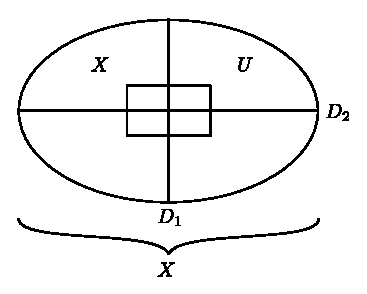
\includegraphics{art4-fig2.eps}
\caption{}
\end{figure}
By\pageoriginale a \textit{neighborhood at infinity} we will mean an open set $U \subset X$ given by \eqref{art4-eq5.4}. By $\bar{U}$ we will mean the polycylinder $|z_i| < \epsilon$ so that 
$$
 U = \bar{U} - \bar{U} \cap D.
$$

\setcounter{definition}{5}
\begin{definition}\label{art4-def5.6}
The `$C^\infty$ log complex' $A^\ast (U, \log \langle D\rangle)$ is the complex of $C^\infty$ forms $\varphi \in A^\ast (U)$ such that
\begin{gather*}
z_1 \ldots z_k \varphi \\
z_2 \ldots z_k d \varphi 
\end{gather*}
are $C^\infty$ in $\bar{U}$.
\end{definition}

Note that $A^\ast (U, \log \langle D \rangle)$ is closed under $d$, and it will follow from Lemma \eqref{art4-lem5.7} that the product of two forms in $A^\ast (U, \log \langle D \rangle )$ is again in the log complex. Thus $A^\ast (U, \log \langle D \rangle)$ is a sub-complex of the full de Rham complex $A^\ast (U)$. Note that $A^\ast (U, \log \langle D \rangle)$ is \textit{not} closed under conjugation.

\setcounter{lemma}{6}
\begin{lemma}\label{art4-lem5.7}
$A^\ast (U, \log \langle D \rangle) = A^\ast (U) \left\{\dfrac{dz_1}{z_1} \ldots , \dfrac{dz_k}{z_k} \right\}$.
\end{lemma}

\begin{proof}
We assume that $k =1$; the general case is similar. Clearly
$$
A^\ast (\bar{U}) \left\{\frac{dz_1}{z_1}, \ldots, \frac{dz_k}{z_k} \right\} \subset A^\ast (U, \log \langle D \rangle).
$$
Conversely, suppose that $\alpha \in A^\ast (U, \log\langle D \rangle)$  and write 
$$
\alpha = \beta \wedge \frac{dz_1}{z_1} + \frac{\gamma}{z_1},
$$
where $\beta$, $\gamma$ do not involve $dz_1$. By the first condition in \eqref{art4-eq5.6}, we may assume that $\beta$, $\gamma$ are $C^\infty$ in $\bar{U}$. Now
$$
d\alpha = \left(\frac{(d \beta \wedge dz_1)}{z_1} + \frac{d\gamma}{z_1} \right) + \frac{\gamma \wedge dz_1}{(z_1)^2}
$$\pageoriginale
and the second condition in \eqref{art4-eq5.6} gives that $\dfrac{\gamma}{z_1} = \delta \in A^\ast (\bar{U})$. Then $\alpha = \beta \wedge \dfrac{dz_1}{z_1} + \delta$ lies in $A^\ast (\bar{U}) \left\{\dfrac{dz_1}{z_1} \right\}$.
\end{proof}

\setcounter{definition}{7}
\begin{definition}\label{art4-def5.8}
The `$C^\infty \log$ complex' $A^\ast (X, \log \langle D \rangle)$ on $X$ is the sub-complex of $A^\ast (X)$ consisting of all $\varphi$ which are in $A^\ast (U, \log \langle D \rangle)$ for all neighborhoods $U$ at infinity.
\end{definition}

To give the global analogue of \eqref{art4-lem5.7}, we consider the line bundles $[D_i] \to \bar{X}$ and choose sections $\sigma_i \in \Gamma (\bar{X}, \cO[D_i])$ with $(\sigma_i) = D_i$ and fibre metrics in $[D_i]$. Setting
\begin{gather*}
\eta_i = \frac{1}{2\pi \sqrt{-1}} \partial \log |\sigma_i|^2,\\
\omega_i = \bar{\partial} \eta_i,
\end{gather*}
it follows (\cf \S \ref{art4-sec2}(b)) that
\setcounter{equation}{8}
\begin{equation}
A^\ast (X, \log \langle D \rangle) = A^\ast (\bar{X}) \{\eta_1, \ldots , \eta_N\}, \label{art4-eq5.9}
\end{equation}
and $\omega_i \in H^2_{DR} (\bar{X})$ is the dual cohomology class of $D_i$.

It will be proved now that the natural map
$$
H^\ast (A^\ast (X, \log \langle D \rangle)) \to H^\ast (A^\ast (X)) \cong H^\ast (X, \bC)
$$
is an isomorphism, and that $A^\ast (X, \log \langle D \rangle)$ has a weight and Hodge filtration inducing a mixed Hodge structure on $H^\ast (X)$.

\medskip
\noindent
(b)~ \textit{The weight filtration and the Poincar\'e residue operator.}

\begin{defi*}
On $A^\ast (X, \log \langle D \rangle)$ we define the weight filtration'\break $W_l = W_l (A^\ast (X, \log \langle D \rangle)$  to be those forms $\varphi$ such that locally at infinity
$$
\varphi \in A^\ast (\bar{U}) \left\{\frac{dz_{i_1}}{z_{i_1}}, \ldots, \frac{dz_{i_l}}{dz_{i_l}} \right\}.
$$
\end{defi*}

Informally, $\varphi$ has weight $l$ if $\varphi$ involves at most $l \dfrac{dz_i}{z_i}s$. Clearly
\setcounter{equation}{9}
\begin{equation}
\left. 
\begin{aligned}
W_l \subset W_{l+1} \;\; & \\
dW_l \subset W_l \;\; & \\
W_l \wedge W_{l'} \subset W_{l+l'}. \;\;
\end{aligned}
\right\}\label{art4-eq5.10} 
\end{equation}\pageoriginale

Note that the definitions of the log complex and weight filtration are local around a point $z \in X$. Thus we may define \textit{complexes} of sheaves on $\bar{X}$
\begin{align*}
& \sA^\ast (\log \langle D \rangle)\\
& \sW_l = W_l (\sA^\ast (\log \langle D \rangle))
\end{align*}
such that  $A^\ast (X, \log \langle D \rangle) = \Gamma (\bar{X}, \sA^\ast (\log \langle D \rangle))$ and similarly for $W_l$. By the usual partition of unity argument, these sheaves have no higher higher cohomology.

Given that $D = D_1 \cup \ldots \cup D_N$, we shall use the following notations:
\begin{align*}
I & = \{i_1, \ldots , i_k\} \subset \{1, \ldots, N\} \; \text{ is an \textit{ index } set;}\\
D_I & = D_{i_1} \cap \ldots \cap D_{i_k},\\
|I| & = k;
\end{align*}
and 
$$
D^{[k]} = \cup_{|I|=k} D_1.
$$

\begin{defi*}
The `Poincar\'e residue operator'
\footnotetext[21]{$A^\ast(\sD^{[k']})$ is the sheaf of $C^\infty$ forms on $D^{[k]}$, sometimes referred to as the \textit{de Bham sheaf}.}
$$
R^{[K]}: \sW_k (\sA^\ast (\log \langle D \rangle)) \to A^{\ast -k} (D^{[k]})\footnotemark[21]{}
$$
is defined by 
\begin{equation}
R^{[k]} \left(\alpha \wedge \frac{dz_{i_1}}{z_{i_1}} \wedge \ldots \wedge \frac{dz_{i_k}}{z_{i_k}} \right)  = \alpha|_{D_I}. 
\label{art4-eq5.11}
\end{equation}
\end{defi*}

The following lemma is easy to verity

\setcounter{lemma}{11}
\begin{lemma}\label{art4-lem12}
\begin{itemize}
\item[(i)] $R^{[k]}$ is well defined and $R^{[k]} (\sW_{k-1}) = 0$; and 

\item[(ii)] $R^{[k]}$ commutes with $d$, $\partial$, and  $\bar{\partial}$.
\end{itemize}
\end{lemma}

Not quite so simple is the \textit{Poincar\'e lemma} in the present context. To explain it, we recall that associated to a complex of sheaves $\sL^\ast = \{\ldots \to \sL^p {\displaystyle{\mathop{\longrightarrow}^d}} \sL^{p+1} \to \ldots \}$\pageoriginale on a space, the \textit{cohomology sheaf}
$$
\sH^\ast (\sL^\ast)
$$
is that sheaf coming from the presheaf
$$
U \longmapsto \text{ cohomology of } \{ \ldots \Gamma (U, \sL^p) {\displaystyle{\mathop{\longrightarrow}^d}} \Gamma (U, \sL^{p+1}) \to \ldots \}.
$$
Thus, \eg, the statement $\sH^q (\sL^\ast) = 0$ for $q>0$ is nothing other than the Poincar\'e lemma. In the situation that we shall encounter, $\sL^\ast$ will be a subcomplex of the de Rham sheaf and will be closed under $d$, $\partial$, and $\bar{\partial}$. We shall denote the various cohomology sheaves by $\sH^\ast_d (\sL^\ast)$, $\sH^\ast_\partial (\sL^\ast)$, $\sH^\ast_{\bar{\partial}}(\sL^\ast)$.

\begin{lemma}\label{art4-lem5.13}
The induced mappings 
\begin{align*}
& R^{[k]}: \sH^\ast_d (\sW_k / \sW_{k-1}) \to \sH^{\ast-k}_d (\sA^\ast (D^{[k]}))\\
& R^{[k]} : \sH^\ast_{\bar{\partial}} (\sW_k / \sW_{k-1}) \to \sH^{\ast-1}_{\partial} (\sA^\ast (D^{[k]}))
\end{align*}
are isomorphisms.\footnote[22]{Since $R^{[k]}$ is surjective, the subtlety here is that there are forms $\alpha \in \sW_k$ with $R^{[k]}\alpha =0$ but $\alpha \not\in \sW_{k-1}$ (\eg $\bar{z} \dfrac{dz}{z}$ on $\bC$.) What must be proved is that these don't matter when we pas to cohomology. The lemma is \textit{false} for $\partial$-cohomology, essentially because we are using $\dfrac{dz}{z}$ and not $\dfrac{d\bar{z}}{z}$ for the long complex.}
\end{lemma}

The proof of \eqref{art4-lem5.13} is essentially the same as the proof of Proposition  \eqref{art4-prop2.18}, and will be omitted.

(c) ~ \textit{de Rham's theorem for the log complex.}

\setcounter{proposition}{13}
\begin{proposition}\label{art4-prop5.14}
The inclusion $A^\ast (X, \log \langle D \rangle) \hookrightarrow A^\ast (X)$ induces an isomorphism on cohomology. Thus
$$
H^\ast (A^\ast X, \log \langle D \rangle) {\displaystyle{\mathop{\longrightarrow}^{\sim}}} H^\ast )(X, \bC).
$$
\end{proposition}

\begin{proof}
Essentially, this proposition is true because it is true locally at infinity by  \eqref{art4-lem5.13}. The easiest way to make this precise is using some homological nonsense.

The basic fact we shall utilize is that if $\sL^\ast = \{\ldots \to \sL^p {\displaystyle{\mathop{\longrightarrow}^d}} \sL^{p+1} \to \ldots \}$ is a complex of sheaves on a space $Y$ and if the cohomology $H^q (Y, \sL^p) =0$ for $q > 0$ then there is a spectral sequence $\{E_r\}$ with 
\begin{gather*}
E_2 = H^\ast (Y, \sH^\ast (\sL^\ast))\\
E^\infty \Rightarrow \text{ cohomology of } \{\ldots \Gamma (Y, \sL^p) {\displaystyle{\mathop{\longrightarrow}^{d}}} \Gamma (Y, \sL^{p+1}) \to \ldots  \}
\end{gather*}\pageoriginale
(\cf \cite{art4-key17}, pages 176-179). As an application, we see that if $\sL^\ast$, $\sK^\ast$ are two complexes of sheaves with $H^q (Y, \sL^\ast) = 0 = H^q (Y, \sK^\ast)$ for $q >0$, and if we are given a morphism
$$
\sL^\ast {\displaystyle{\mathop{\longrightarrow}^{\psi}}} \sK^\ast
$$
of complexes of sheaves such that cohomology sheaf map
$$
\psi_\ast : \sH^\ast (\sL^\bigdot) {\displaystyle{\mathop{\longrightarrow}^{\sim}}} \sH^\ast (\sK^\bigdot)
$$
is an isomorphism, then the global cohomology map
$$
\frac{\ker \{\Gamma (Y, \sL^p) \to \Gamma (Y, L^{p+1})\}}{d \Gamma (Y, L^{p+1})} \to \frac{\ker \{\Gamma (Y, \sK^p) \to \Gamma (Y, \sK^{p+1})\}}{d\Gamma (Y, \sK^{p-1})}
$$
is also an isomorphism.

We shall apply this principle taking $Y =\bar{X}$, $\sL^\ast = \sA^\ast (\log \langle D \rangle)$, and $\sK^\ast = j_\ast (\sA^\ast (X))$, where $j:X \hookrightarrow\bar{X}$ is the inclusion mapping. Note that $\Gamma (\bar{X}, \sA^\ast (\log \langle D \rangle)) = A^\ast (X, \log \langle D\rangle)$  and $\Gamma (\bar{X}, j_\ast (\sA^\ast (X))) = A^\ast (X)$. Proposition \ref{art4-prop5.14} consequently follows from the
\end{proof}

\begin{lemma*}
The induced mapping
$$
\sH^\ast (\sA^{\ast} (\log \langle D \rangle)) {\displaystyle{\mathop{\longrightarrow}^{\sim}}} \sH^{\ast} (j_\ast (\sA^\ast (X)))
$$
is an isomorphism.
\end{lemma*}

\begin{proof}
The question is local in a neighborhood $U$ at infinity give by \eqref{art4-eq5.4}. Let
$$
\bC \left\{\frac{dz_1}{z_1}, \ldots, \frac{dz_k}{z_k} \right\} = \bC \left\{ \left\{\frac{dz_i}{z_i} \right\} \right\}
$$
be the free differential graded algebra generated by $\dfrac{dz_1}{z_1} ,\ldots,\dfrac{dz_k}{z_k}$ and having differential $d=0$. There is a commutative triangle
$$
\xymatrix@R=1.5cm@C=.6cm{
A^\ast (U, logs \langle D \rangle) \ar[rr] && A^\ast (U)\\
& \bC \left\{\frac{dz_1}{z_1} , \ldots , \frac{dz_k}{z_k} \right\}  \ar[ur]_v \ar[ul]_{\mu} &
}
$$
\pageoriginale
of complexes, and $v_\ast$ is an isomorphism on cohomology by the usual de Rham theorem. Thus it will suffice to show that $\mu_{\ast}$ is an isomorphism on cohomology.

There is an obvious weight filtration $W_l \left(\bC \left\{\left\{\dfrac{dz_i}{z_i} \right\} \right\} \right)$ such that 
$$
\mu \left[W_l \left(\bC\left\{ \left\{ \frac{dz_i}{z_i}\right\}  \right\}\right) \right] \subset W_l (A^\ast (U, \log \langle D \rangle)).
$$
Moreover, there is a commutative triangle
$$
\xymatrix@R=1.5cm@C=.6cm{
\frac{W_l (A^\ast (U, \log \langle D \rangle))}{W_{l-1} (A^\ast (U, \log \langle D \rangle))}  \ar[rr]^-{R^{[K]}} && A^{\ast =k } (D^{[k]} \cap U)\\
& \frac{W_l \left(\bC \left\{ \left\{ \frac{dz_i}{z_i} \right\} \right\}\right)}{W_{l-1} \left(\bC \left\{ \left\{ \frac{dz_i}{z_i}  \right\} \right\} \right)} \ar[ur]_-{\beta = \text{Poincar\'e residue}} \ar[ul]_-{\alpha} & 
}
$$
where $\beta_\ast$ is obviously an isomorphism on cohomology, and $R^{[k]}_\ast$ is also an isomorphism by Lemma \eqref{art4-lem5.13}. (This is the main step in the proof). Thus $\alpha_\ast$ is an isomorphism on cohomology. Using this it follows inductively on $l$ that
$$
\mu : W_l \left[ \bC \left\{ \left\{ \frac{dz_i}{z_i} \right\} \right\} \right] \to W_l (A^\ast (U, \log \langle D \rangle))
$$
induces\pageoriginale an isomorphism on cohomology. For $l=k$, we obtain our lemma.
\end{proof}

\begin{remark*}
Lemma \ref{art4-lem5.13} plus the same method of proof gives the 
\end{remark*}

\setcounter{coro}{14}
\begin{coro}\label{art4-coro5.15}
The residue mapping $R^{[k]} : W_k / W_{k-1} \to A^{\ast -k} (D^{[k]})$ induces isomorphism on both $d$ and $\bar{partial}$ cohomology.
\end{coro}

\medskip
(d)~ \textit{The weight and Hodge filtration on cohomology.} On the $C^\infty$ log complex $A^\ast (X, \log \langle D \rangle)$ we have defined the weight filtration, $W_l$ in \S \ref{art4-sec5}(b), and we now define the \textit{Hodge filtration by}
\setcounter{equation}{15}
\begin{equation}
F^p A^{\ast} (X, \log \langle D \rangle) = \oplus_{i \geqslant p} A^{i,\ast} (X, \log \langle D \rangle) .
\label{art4-eq5.16}
\end{equation}
The weight and Hodge filtrations induce filtrations on the cohomology $H^\ast (A^\ast (\log \langle D \rangle)) \cong H^\ast (X, \bC)$, and it is to be proved that (with suitable indexing!) this gives a mixed Hodge structure.

\setcounter{proposition}{16}
\begin{proposition}\label{art4-prop5.17}
The weight filtration $W_n \{H^\ast (X, \bC)\}$ is defined over $\bQ$.
\end{proposition}

\begin{proof}
We begin with a preliminary remark. Suppose that $\varphi \in W_l (A^\ast (X, \log \langle D \rangle))$ is a closed form of filtration level $l$. Then the Poincar\'e residue
$$
R^{[l]} \varphi \in A^{\ast -l} (D^{[l]})
$$
is a closed form giving a cohomology class in $H^{\ast-1} (D^{[l]}, \bC)$. If this class is zero, then by Corollary \ref{art4-coro5.15} we may find $\theta \in W_l$ such that $\varphi -d \theta \in W_{l-1}$.

To prove the proposition, we take a closed form $\varphi\in A^{\ast} (X, \log \langle D \rangle)$. Then
$$
R^{[n]} \varphi \in H^\ast (D^{[n]} , \bC)
$$
is well defined. If $\varphi \in W_{n-1}$, then $R^{[n]} \varphi =0$, and conversely if $R^{[n]} \varphi$ is zero in cohomology, then by the above remark we may find $\theta \in A^\ast (X, \log \langle D \rangle)$ such that $\varphi - d \theta \in W_{n-1}$. Repeating this argument we find that 
\setcounter{equation}{17}
\begin{equation}
W_l \{H^\ast (X,\bC)\} = \{\varphi \in H^\ast (X, \bC): R^{[n]} \varphi = \ldots = R^{[l+1]} \varphi =0\} \label{art4-eq5.18}
\end{equation} 
where, on the right hand side, the $R^{[v]}\varphi$ are taken in $H^\ast (D^{[v]}, \bC)$. With\pageoriginale the description \eqref{art4-eq5.18}, it is clear that the weight filtration $W_l \{H^\ast (X, \bC)\}$ is defined over $\bQ$.

Now consider the filtration
\begin{equation}
W^{-l} = W_l (A^\ast (X, \log \langle D \rangle))
\label{art4-eq5.19}
\end{equation}
on the log complex. The indices have been reversed in order to give \textit{decreasing} filtration,
$$
\ldots \supset W^{-l} \supset W^{-l+1} \supset \ldots,
$$
sot that we may consider the spectral sequence (=s.s.) of a filtered complex \cite{art4-key17}. Accordingly, there is a s.s. $\{E_r\}$ such that $E_\infty$ is the associated graded to the weight filtration on $H^\ast (X, \bC)$ and 
$$
E_1 = H^\ast (W^{-l}/ W^{-l+1}).
$$
\end{proof}

\setcounter{lemma}{19}
\begin{lemma}\label{art4-lem5.20}
The Hodge filtration $\{F^p\}$ induces a Hodge structure of pure weight $k+l$ on $H^k (W^{-l} / W^{-l+1})$.
\end{lemma}

\begin{proof}
Using the obvious notations,
$$
F^p (W^{-l} / W^{-l+1}) \cong (\oplus_{i\geqslant p} W^{i,\ast}_l)/ W_{l-1}.
$$
The Poincar\'e residue operator induces
$$
F^p (W^{-l}/ W^{-1+1}) {\displaystyle{\mathop{\longrightarrow}^{R^{[l]}}}} F^{p-l} (A^{\ast} (D^{[l]})).
$$
Applying Corollary \ref{art4-coro5.15}, it follows that 
$$
H^k (W^{-1}/ W^{-l+1}) \cong H^{k-1} (D^{[l]})
$$
is a morphism of Hodge structures of type $(-l, -l)$.
\end{proof}

\begin{lemma}\label{art4-lem5.21}
The mapping $d_1 : E_1 \to E_1$ is a morphism of Hodge structures.
\end{lemma}

\begin{proof}
Using the isomorphism
$$
E_1 \cong \oplus_I H^\ast (D_I), 
$$
we shall prove using \eqref{art4-eq2.19} that $d_1$ is given by Gysin mappings 
$$
H^\ast (D_{i_1\ldots i_l}) \to H^{\ast+2} (D_{i_1 \ldots i_{l-1}})
$$
A class $\varphi \in H^\ast (W^{-l}/ W^{-l+1})$ may be represented by a form $\varphi \in W_l (A^\ast (X, \log \langle D \rangle))$ such that $R^{[l]} d \varphi = d R^{(l)} \varphi =0$. Then by definition
$$
d_1 \varphi = R^{[l-1]} d_\varphi,
$$\pageoriginale
since $d_1$ is the coboundary map arising from the exact sequence of complexes
$$
0 \to W_{l-1}/ W_{l-2} \to W_l /W_{l-2} \to W_l / W_{l-1} \to 0.
$$

Write $\eta_I = \eta_{i_1} \wedge \ldots \wedge \eta_{i_l}$ and $\varphi =\sum\limits_{|i| =l} \eta_I \wedge \varphi_I$. Then by an obvious computation
$$
R^{[l-1]} d \varphi|_{D_{i_1} \ldots i_{l-1}} = \sum\limits_{j} \pm \{\omega_j \wedge \varphi_{i_1 \ldots i_{l - 1} j} + \eta_j \wedge d \varphi_{i_1 \ldots i_{l-1} j}\},
$$
which is just the Gysin mapping according to \eqref{art4-eq2.19}.
\end{proof}

\setcounter{coro}{21}
\begin{coro}\label{art4-coro5.22}
The weight and Hodge filtrations on $A^\ast (X, \log \langle D \rangle)$ induce a mixed Hodge structure on $E_2$.
\end{coro}

\begin{proof}
This follows from Lemmas \ref{art4-lem5.20}, \ref{art4-lem5.21} and Corollary \ref{art4-coro1.15}.
\end{proof}

The main remaining step in the proof of Deligne's theorem is to show that the spectral sequence in question degenerates at $E_2$. This will be proved in the next section.

\medskip
\noindent
(e)~ \textit{Completion of the proof of Theorem \ref{art4-thm5.1}.}     

\begin{enumerate}
\item[(i)] \textit{Degeneration of the spectral sequence.}

We continue the discussion of \S \ref{art4-sec5}(c). In case $D$ is smooth, the weight filtration is just $W_0 \subset W_1$ and consequently $E_2 = E_\infty$. The crucial case is when $D= D_1 \cup D_2$, and we shall check here that $d_2 = 0 -$this will suffice to make clear how the general argument goes.

Let $\alpha$ be a class in 
$$
E^{-2}_1 = H^\ast (W_{-2}/ W_1) \cong H^{\ast-2} (D_1 \cap D_2)
$$ 
(\cf \ref{art4-coro5.15}). We may assume that $\alpha$ is represented by a closed $C^\infty(p,q)$ form on $D_1 \cap D_2$. Let $\tilde{\alpha}$ be a $C^\infty$ extension of $\alpha$ and $\eta_1$, $\eta_2$ as in \eqref{art4-eq5.9}. Then
$$
A' = \eta_1 \wedge \eta_2 \wedge \tilde{\alpha}
$$
gives a form in $W_2 \{A^\ast (X, \log \langle D \rangle ) \}$ with 
$$
R^{[2]} A' = \alpha.
$$
If\pageoriginale  $d_1 \alpha = 0$, then, referring to the proof of Lemma \eqref{art4-lem5.21}. we may find forms $\beta_i$ on $D_i$ such that
\setcounter{equation}{22}
\begin{equation}
\left.
\begin{aligned}
& R^{[1]} (dA')_{D_1} = \eta_2 \wedge d \tilde{\alpha} + \omega_2 \wedge \tilde{\alpha}|_{D_2} = d \beta_1,\\
& R^{[1]} (dA')_{D_2}  =\eta_1 \wedge d\tilde{\alpha} + \omega_1 \wedge \tilde{\alpha}|_{D_1} = d \beta_2.
\end{aligned}
 \right\}
\label{art4-eq5.23}
\end{equation}
Moreover, we may choose the $\beta_i$ to have type $(p+q+1,0) + \ldots + (p +1,q)$  (\cf \eqref{art4-lem2.10}). Setting $B' = - (\eta_1 \wedge \tilde{\beta}_1 + \eta_2 \wedge \tilde{\beta}_2)$  where the $\tilde{\beta_i}$ are $C^{\infty}$ extensions of $\beta_1$, $\beta_2$, we find the relations
\begin{equation}
\left.
\begin{array}{c}
R^{[2]} (A' + B') =\alpha\\
R^{[2]} (d (A'+B')) = R(^{[1]} (d (A'+B')) =0\\
d(A'+B') \in F^{p+2} A^\ast (X, \log \langle D \rangle).
\end{array}
\right\} \label{art4-eq5.24}
\end{equation}

Now we may repeat the same argument using $\bar{\eta_1},\; \bar{\eta_2}$ and solving the equations \eqref{art4-eq5.23} emphasizing the opposite direction in the Hodge filtration. This leads to $A''$, $B''$ satisfying
\begin{equation}
\left.
\begin{array}{c}
R^{[2]} (A'' + B'') =\alpha\\
R^{[2]} (d (A''+B'')) = R(^{[1]} (d (A''+B'')) =0\\
d(A''+B'') \in F^{p+2} A^\ast (X, \log \langle D \rangle).
\end{array}
\right\} \label{art4-eq5.24}
\end{equation}
Since $\deg [d(A'+ B')] = p + q +3$, equations \eqref{art4-eq5.24} and \eqref{art4-eq5.25} say exactly that $d_2 \alpha \in E^0_2$\footnote[23]{Recall that $d_2 : E_2 -2 \to E^0_2$.} has total degree $p+q+3$ and is in 
$$
F^{p+2} (E^0_2) F \cap F^{q+2} (E^0_2) = 0,
$$
since $E_2$ has a mixed Hodge structure by \eqref{art4-eq5.22}. Thus $\alpha_2 \alpha = 0$.

\begin{remark*}
As was the case in the proof of Lemma \eqref{art4-eq4.7}, this proof is simply an application of the principle of two types as discussed at the end of \S \eqref{art4-sec2} (a).
\end{remark*}

\item[(ii)] \textit{Tying up loose ends.}

Given $X$, we have chosen a smooth completion $\bar{X}$ of $X$, defined the log complex $A^\ast (X, \log \langle D \rangle)$ with weight filtration $W_n$ and Hodge filtration $F^p$, and proved that 
\begin{align*}
& H^\ast (A^\ast (X, \log \langle D \rangle )) \cong H^\ast (X, \bC);\\
& \text{the filtration $W_n, \; F^p$ induce a mixed} \\
& \text{Hodge structure on $H^\ast (A^\ast (X, \log \langle D \rangle))$.}
\end{align*}\pageoriginale
Moreover, Corollaries \eqref{art4-coro5.2} and \eqref{art4-5.3} follow immediately from the definitions of $W_n$ and \eqref{art4-coro5.20}. It remains, therefore, to prove independence of our construction from the smooth completion $\bar{X}$ and functoriality.

Observe first that, given a diagram
\begin{equation}
\vcenter{
\xymatrix{
Y \ar@{^{(}->}[r] \ar[d]_-f & \bar{Y} \ar[d]^-{\overline{f}}\\
X \ar@{^{(}->}[r] & \bar{X}}}\label{art4-eq5.26}
\end{equation}
then $\overline{f}^\ast : A^\ast (X, \log \langle D \rangle) \to A^{\ast} (Y, \log \langle D \rangle)$ commutes with the weight and Hodge filtrations. Given smooth completions $\overline{X}_1, \overline{X}_2$ of $X$, by \cite{art4-key29} there exists a smooth completion $\overline{X}_3$ and a diagram
$$
\xymatrix{
& \overline{X}_3 \ar[dl] \ar[dr]&\\
\overline{X}_1 & \text{\boldmath$\cup$}  & \overline{X}_2 \\
& X \ar@{}[ul]|{\displaystyle{\rotatebox{35}{\boldmath$\cup$}}} \ar@{}[ur]|{\displaystyle{\rotatebox{-35}{\boldmath$\cup$}}} & 
}
$$
and independence of the smooth compactification follows. Given a morphism $ Y {\displaystyle{\mathop{\longrightarrow}^f}}$ using \cite{art4-key29} again we may find a diagram \eqref{art4-eq5.26} and this implies functoriality. 
\end{enumerate}

\section{Application of mixed Hodge structures.}\label{art4-sec6}
(a)~ \textit{Application to moduli}. Let $X, \; S$ be smooth quasi-projective varieties and $f: X \to S$ a smooth, proper mapping. Setting $V_s = f^{-1} (s) (s \in S)$, we may think of $X$ as an algebraic family $\{V_s\}_{s \in S}$ of smooth, projective varieties with algebraic parameter space $S$. Pick a base point $s_0 \in S$ and set $V = V_{s_0}$. The fundamental group $\pi_1 (S, s_0)$ acts on the cohomology $H^n (V, \bQ)$, and we let
$$
I^n  = H^n (V, \bC)^{\pi_1}
$$
by the \textit{invariant part} of the cohomology under this action. Note that for each point $s \in S$ there is a well-defined inclusion
$$
i_s : I^n \hookrightarrow H^n (V_s, \bC)
$$\pageoriginale
obtained by ``transporting'' $I^n$ to $V_s$ along some path from $s_0$ to $s$.

\setcounter{proposition}{0}
\begin{proposition}[\cf Corollary 4.1.2 of \cite{art4-key13}]\label{art4-prop6.1}
$I^n \subset H^n (V, \bC)$ has an induced Hodge structure, and the inclusions $i_s$ are all morphisms of Hodge structures. 
\end{proposition}

\begin{remark*}
In other words, if $\varphi$ is an invariant cohomology class and if in each $H^n (V_s, \bC)$ we decompose $\varphi$ into $(p,q)$ type
$$
\varphi = \sum\limits_{p+q = n} \varphi_{p,q} (s),
$$
then the $\varphi_{p,q} (s)$ are \textit{constant in $s$}. In particular, if $\varphi$ is of fixed type $(p,q)$ at one point $s \in S$, then $\varphi$ is everywhere of the same $(p,q)$ type.
\end{remark*}

In \cite{art4-key19}, Proposition \ref{art4-prop6.1} was proved for an arbitrary variation of Hodge structure $\bH \to S$ with compact base space $S$. Using the  results of the second author \cite{art4-key41} discussed in \S \ref{art4-sec9} below, \eqref{art4-prop6.1} may be proved for an arbitrary variation of Hodge structure $\bH \to S$ with an algebraic variety as base space (\cf \S \ref{art4-sec10}).

\begin{proof}
According to Deligne's degeneration theorem discussed in \S \eqref{art4-sec2}(a), the image of 
$$
H^n (X, \bC) {\displaystyle{\mathop{\longrightarrow}^\rho}} H^n (V, \bC)
$$
is exactly $I^n$. Note that $i_s (I^n)$ is then the image of 
$$
H^n (X, \bC) {\displaystyle{\mathop{\longrightarrow}^{\rho_s}}} H^n (V_s, \bC)
$$
for all $s \in S$. Let $\overline{X}$ be a smooth compactification of $X$. In the diagram 
$$
\xymatrix{
H^n (X, \bC) \ar[r]^\rho & H^n (V_s \bC)\\
H^n (\bar{X}, \bC) \ar[u] \ar[ur]_{\overline{\rho}}
}
$$
we will show that
\setcounter{equation}{1} 
\begin{equation}
\text{image } \rho = \text{image } \bar{\rho} . 
\label{art4-eq6.2}
\end{equation}\pageoriginale
If this is done, then because $\bar{\rho}$ is a morphism of Hodge structures,
$$
I^n \cong H^n (\bar{X}, \bC) / \ket \bar{\rho}
$$
will have an induced Hodge structure. Since $\ker \bar{\rho} = \ker \bar{\rho}_s$ for all $s$, the inclusion $i_s$ will be morphisms of Hodge structures and our proposition is proved.
\end{proof}

According to Theorem \ref{art4-thm5.1}, the cohomology $H^n(X, \bC)$ has a \textit{functorial mixed} Hodge structure $\{W_n, F^p, H^n (X, \bC)\}$ with
\begin{equation}
W_n (H^n (X, \bC)) = \image \{H^n (\bar{X}, \bC) \to H^n (X, \bC) \}. \label{art4-eq6.3}
\end{equation}
Since $H^n(\bar{X}, \bC)$ and $H^n (V, \bC)$ have mixed Hodge structures of pure weight $n$ and all maps are morphisms of mixed Hodge structures, our assertion \eqref{art4-eq6.2} follows from \eqref{art4-eq6.3} and the strictness Lemma \eqref{art4-eq1.10}.

(b) \textit{A direct proof of a result of Deligne about meromorphic forms on projective varieties.} Let $V$ be a compact K\"ahler manifold. It is well known that 
\begin{equation}
\left.
\begin{aligned}
 & \text{~(i) every holomorphic form on $V$ is closed;}\\
 & \text{(ii) a non-zero holomorphic form is not exact.} 
\end{aligned}
\right\}\label{art4-eq6.4}
\end{equation}

Clearly (ii) $\Rightarrow$ (i), and (ii) may be most easily seen as follows: Suppose that $\varphi \not\equiv 0$ is a holomorphic $q$-form and $\varphi = d \eta$ for a $C^\infty$ form $\eta$. Letting $\omega$ be the K\"ahler form, by Stokes' theorem, and because $d\omega = 0$,
$$
0 < (\sqrt{-1})^{q^2} \int\limits_v \varphi \wedge \bar{\varphi} \wedge \omega^{n-q} = (\sqrt{-1})^{q^2} \int\limits_v d (\eta \wedge \bar{\varphi} \wedge \omega^{n-q}) = 0,
$$
a contradiction. In \cite{art4-key13} Deligne proved the following generalization of \eqref{art4-eq6.4}:

\setcounter{proposition}{4}
\begin{proposition}\label{art4-eq6.5}
Let $D \subset V$ be a divisor with normal crossings and $\varphi \in \Gamma (V, \Omega^q (\log \langle D \rangle))$ a meromorphic $q$-form having a logarithmic singularity on $D$. Then
\begin{itemize}
\item[(i)] $d\varphi = 0$, and 

\item[(ii)] if $\varphi =0$ in $H^q (V - D, \bC)$, then $\varphi \equiv 0$.
\end{itemize}
\end{proposition}

\begin{proof}
We shall\pageoriginale give a proof similar to the special case discussed above. Observe that the result is not changed if we replace $D$ by $D + H$, where $H$ is a suitable hypersurface section relative to a projective embedding of $V$. Thus we are free to make $D$ as ample as we wish.

We first show that (i) $\Rightarrow$ (ii). Setting $u = V - D$, if 
$$
\varphi \in\Gamma (V, \Omega^q (\log \langle D \rangle))
$$
is zero in $H^q (u, \bC)$, then taking $u$ to be affine, we have by the \textit{algebraic de Rham theorem} \cite{art4-key26} that
\begin{equation}
\varphi =d \eta \label{art4-eq6.6}
\end{equation}
where $\eta$ is meromorphic on $V$ and holomorphic on $U$. The obstruction to lowering the order of pole of $\eta$ along $D$ to \textit{one} are in cohomology groups (\cf \S \ref{art4-sec10} in \cite{art4-key20})
$$
H^\ast (V, \Omega^\bigdot_V \otimes \cO [\mu D]) \quad (\ast > 0, \mu > 0), 
$$
and these may be made zero by making $D$ more ample. Thus we may assume that $\eta$ has a pole of order one on $D$, and then
$$
\eta \in \Gamma (V, \Omega^{q-1} (\log \langle D \rangle))
$$
by \eqref{art4-eq6.6}. Applying (i), $0 = d \eta = \omega$ which gives (ii).

We now prove (i). The \textit{Poincar\'e residue} (\cf \S \ref{art4-sec5}(b)) $R (\varphi)$ is a holomorphic $q -1$ form on $D$, and thus $d R (\varphi)=0$ by the usual result on K\"ahler manifolds. Thus
$$
R(d \varphi) = d (R \varphi) =0,
$$
and so $d \varphi$ is holomorphic on $V$. Let $T_\epsilon$ be an $\epsilon$-tube around $D$. Then
\begin{align*}
0 & < (\sqrt{-1})^q \int_v d\varphi \wedge d \bar{\varphi} \wedge \omega^{n-q-1} \; (\text{since $d \varphi$ is holomorphic on $V$})\\
& = (\sqrt{-1})^q \lim\limits_{\epsilon \to 0} \int_{\partial T_\epsilon} \varphi \wedge \overline{d \varphi} \wedge \omega^{n-q-1} \; \text{(Stokes' theorem)}\\
& = \dfrac{(-1)^q}{2\pi \sqrt{-1}} \int_D R (\varphi) \wedge \overline{d\varphi} \wedge \omega^{n-q-1} \text{ (by residue formula)}\\
& = 0,
\end{align*}
since $R (\varphi)$ has type $(q-1, 0)$ and $\overline{d \varphi}$ has type $(0, q +1)$.
\end{proof}

\noindent
(c)~ \textit{Intermediate Jacobians.}\footnote[24]{The general reference fo this section is \cite{art4-key22}, whose terminology and notations we shall follow. Intermediate Jacobians are also discussed in \cite{art4-key36}.} Let $V$ be a smooth projective variety of dimension $n$ and
$$
T (V) = \otimes^n_{q=1} T_q (V)
$$
\textit{the intermediate Jacobian} of $V$\footnote[25]{$T_q (V) F^q H^{2q-1} (V-\bC) / H^{2q+1} (V, \bC) / H^{2q-1} (V, \bZ)$, so that $T_1 (V) \cong H^1 (V, \cO)/ H^1 (V,\bZ)$ and $T_{n}(V) = Alb (V)$.} If $\sA (V)$ are the algebraic cycles on $V$ which are algebraically equivalent to zero and taken modulo rational equivalence, then one has the \textit{Abel-Jacobi mapping}
$$
\varphi : \sA (V) \to T (V).
$$
The image $\varphi \{\sA (V)\}$ is an abelian subvariety $I^0(V)$, and an outstanding problem is to (i) describe $I^0(V)$ algebro-geometrically and (ii) prove that, up to isogeny, $I^0_q (V)$ is the dual abelian variety $\widehat{I^0_{n-q+1} (V)}$ to $I^0_{n-q+1} (V)$. Using Deligne's theory, it is possible to do this in one significant new case, which shall now be discussed.

To explain this result, we recall from \S 1 of \cite{art4-22} the notion of \textit{incidence equivalence}, and let $\sQ (V) \subset \sA (V)$ be algebraic cycles which are incidence equivalent to zero. The quotient
$$
\sA (V)/ \sQ (V) = \Pic^0 (V)
$$
was termed in \cite{art4-key22} the identity component of the \textit{(algebraic) Picard variety} of \textit{V. Abel's theorem} (loc. cit, \S 3) gives a factorization
\setcounter{equation}{6}
\begin{equation}
\vcenter{
\xymatrix@R=1.5cm@C=.6cm{ 
\sA(V) \ar[rr]^\varphi \ar[dr]_-{\rho} && I^{0}(V) \ar[dl]^-{\psi}\\
& \Pic^0(V) &}}\label{art4-eq6.7}
\end{equation}
It is conjecturally the case that (i) $\psi$ is an isogeny, and (ii) that the duality relation
\setcounter{equation}{7}
\begin{equation}\label{art4-eq6.8}
\Pic^0_q (V) \cong \widehat{\Pic^0_{n-q+1} (V)}
\end{equation}
is valid upto isogeny. We shall prove that this is so when
\footnotetext[26]{Examples of such $V$ are complete intersections in $\bP^N$. The reason for assuming \eqref{art4-eq6.9} is that all of $H^{2m+1} (V, \bQ)$ is \textit{primitive} (\S 2), and thus the cup-product $H^{2m+1} (V, \bQ) \otimes H^{2m+1} (V, \bQ) \to \bQ$ is \text{non-degenerate} on any sub-Hodge structure of $H^{2m+1} (V, \bQ)$.}
\begin{equation}
\left.
\begin{array}{c}
dim V = 2 m +1 \text{ is odd}\\
H^{2q+1} (V, \bC) = 0 \text{ for } q \neq m\footnotemark[26]{} .
\end{array}
\right\}\label{art4-eq6.9}
\end{equation}\pageoriginale

\begin{proof}
We shall first discuss a special case. Let $\{Z_s\}_{s \in S}$ \textit{be an algebraic family} of $m$-dimensional subvarieties $Z_s \subset V$ with smooth, projective parameter space $S$, and which is in \textit{general position} so that the \textit{incidence divisors}
$$
D_s = \{s' \in S: Z_{s'} \cap Z_s \neq \emptyset\}
$$
are defined. The correspondences
\begin{equation*}
\vcenter{
\xymatrix{
s \ar[r] \ar[d] & Z_s \\
D_s & }}
\end{equation*}
induce mappings 

\begin{equation}
\vcenter{
\xymatrix{
\text{Alb}(S) \ar[r]^-{\varphi} \ar[d]^-{\eta} & I^0_m(V) \ar@{-->}[dl]^-{\psi}\\
\Pic^0_1 (S) &}} \label{art4-eq6.10}
\end{equation}
where the factorization $\eta= \psi^\circ \varphi$  is a consequence of Abel's theorem (\S 3 of \cite{art4-key22}). The homology intersection relation
\begin{equation}
(\varphi_\ast (\alpha), \varphi_\ast (\beta))_V = \pm (\alpha, \eta_\ast (\beta))_S (\alpha, \beta \in H_1 (S, \bZ)) \label{art4-eq6.11}
\end{equation}
is easy to verity, and it follows from \eqref{art4-eq6.10} and \eqref{art4-eq6.11} that up to isogeny 
\begin{equation}
\left\{
\begin{aligned}
&\ker \varphi = \ker \eta\\
&\text{ in \eqref{art4-eq6.10}}
\end{aligned}
\right\}
\Leftrightarrow 
\left\{
\begin{aligned}
&\text{the intersection pairing}\\
&\text{is non-singular on}\\
&\varphi_\ast [H_1 (S, \bQ)]
\end{aligned}
\right\}.
\label{art4-eq6.12}
\end{equation}
Now\pageoriginale $\varphi_\ast [H_1 (X, \bC)]$ is a sub-Hodge structure of $H_{2m+1} (V, \bQ)$, and consequently the intersection pairing is non-singular on $\varphi_\ast [H_1(S,\bC)]$, since $H^{2m+1} (V, \bC)$ is all primitive by the assumption \eqref{art4-eq6.9}. Thus $\ker \varphi^0 = \ker \eta^0$ in this case.

In general, the point is that if $\{Z_s\}_{s \in S}$ is any algebraic family of algebraic $m$-cycles on $V$, then 
$$
\varphi_\ast: H_1 (S, \bC) \to H_{2m+1} (V, \bC)
$$
is a morphism of mixed Hodge structures of type $(m,m)$ and, as a result, the intersection pairing is non-degenerate on
$$
\varphi_\ast [H_1 (\sA(V), \bC)] \subset H_{2m+1} (V, \bC).
$$
Now the same argument as before may be applied to give our desired conclusion.
\end{proof}

\section{Hyperbolic complex analysis and the period mapping.}\label{art4-sec7}
(a) \textit{General commments: the Ahlfors lemma.} Hyperbolic complex analysis is the study of holomorphic mappings into \textit{negatively curved complex manifolds}; \ie complex manifolds $M$ having an Hermitian metric $ds^2_M$ whose \textit{holomorphic sectional curvatures} $K_M (\zeta)$ ($\zeta \in T (M) =$ holomorphic tangent bundle of $M$) satisfy
\footnotetext[27]{The general philosophy and uses of hyperbolic complex analysis are discussed in the monograph \cite{art4-key34} by Kobayashi, and the paper \cite{art4-key48} by $Wu$, both of which contain the relevant definitions and differential-geometric formulas.}
\setcounter{equation}{0}
\begin{equation}\label{art4-eq7.1}
K_M (\zeta) \leqslant - A < 0\footnote[27]{}
\end{equation}
If $N \subset M$ is a complex submanifold with induced metric $ds^2_N$, then for $\zeta \in T (N)$,
\begin{equation}
K_N (\zeta) = K_M (\zeta) - |S(\zeta)|^2, 
\label{art4-eq7.2}
\end{equation}
where $S (\zeta)$ is the \textit{second fundamental form} of $N$ in $M$. In particular, $N$ is negatively curved if $M$ is, and this is one of the two reasons why hyperbolic complex analysis works so well, the other being the Ahlfors Lemma \ref{art4-lem7.7} below.

Let $\Delta = \{z \in \bC : |z| < 1\}$ be the unit disc and define a \textit{pseudometric} on $\Delta$ to be given by 
\begin{equation}
h(z) dz d\bar{z}, \label{art4-eq7.3}
\end{equation}
where\pageoriginale $h(z)$ is $C^\infty$ on $\Delta$ and $h(z) >0$ on $\Delta -R$, for some discrete subset $R$ of $\Delta$. The \textit{Gaussian curvature} and \textit{Ricci form} are defined by
\begin{align}
& K(h) = - \frac{1}{2h} \frac{\partial^2 \log h}{\partial z \partial \bar{z}} \notag\\
& \Ric (\omega) = \frac{\sqrt{-1}}{4} \left( \frac{\partial^2 \log h}{\partial z \partial \bar{z}}\right) dz \wedge d\bar{z} = - K (h) \omega;  \label{art4-eq7.4}
\end{align}
here $\omega = \dfrac{\sqrt{-1}}{2} h dz \wedge d\bar{z}$ is the \eqref{art4-def1.1} form associated to the metric.

The rules (\cf \cite{art4-key24} for further discussion),
\begin{align*}
& \Ric (e^\mu \omega) = \frac{\sqrt{-1}}{4} (\partial \bar{\partial} \mu) + \Ric (\omega)\\
& \Ric (f^\ast\omega) = f^\ast \Ric (\omega) \qquad (f: \Delta \to \Delta \text{ holomorphic})
\end{align*}
afford easy manipulation of the Gaussian curvatures.

If $f : \Delta \to M$ is a non-constant holomorphic mapping into a negatively curved complex manifold $M$, then by \eqref{art4-eq7.2} $f^\ast ds^2_M$ is a pseudometric on $\Delta$, whose Gaussian curvature $K$ satisfies
\footnotetext[28]{The pseudo-metric $\dfrac{1}{A} f^\ast (ds^2_M)$ has Gaussian curvature $K \leqslant -1$, and in this way we may always assume that $A =1$ in \ref{art4-eq7.1}. The points $z_0 \in R$ where $h(z_0) = 0$ should be thought of as having $K (z_0) = - \infty$.}
\begin{equation}
K \leqslant - A < 0.\footnotemark[28]{}
\label{art4-eq7.5}
\end{equation}
The Ahlfors lemma compares a general pseudo-metric satisfying \eqref{art4-eq7.5} to the \textit{Poincar\'e metric}
\begin{equation}
\left.
\begin{array}{c}
ds^2_P = \pi (z) dzd\bar{z}= \frac{dzd\bar{z}}{(1-|z|^2)^2}\\
\Ric \left(\frac{\sqrt{-1}}{2} \pi (z) d z \wedge d\bar{z} \right) = \frac{\sqrt{-1}}{2} \pi (z) dz \wedge d \bar{z}
\end{array}
\right\}\label{art4-eq7.6}
\end{equation}
Despite its simplicity, it is one of the most powerful and subtle tools available in the study of holomorphic mappings.

\setcounter{lemma}{6}
\begin{lemma}[Ahlfors]\label{art4-lem7.7}
Given a pseudo-metric $h(z)dzd\bar{z}$ on $\Delta$ whose Gaussian curvature satisfies $K(z) \leqslant -1$, then $h (z) \leqslant \pi (z)$.\footnote[29]{The invariant form of the \textit{Schwarz lemma} \cite{art4-key28}, due to Pick, states that if $f : \Delta \to \Delta$ is a holomorphic mapping, then $f^\ast (ds^2_P) \leqslant^2_P$, or equivalently
$$
\dfrac{|f'(z)|^2}{(1 -|f(z)^2|)^2} \leqslant \frac{1}{(1-|z|)^2};
$$
this follows from the Ahlfors lemma taking $h(z) dz d \bar{z} = f^\ast (ds^2_P)$. Note that the proof of \eqref{art4-lem7.7} is quite similar to the proof of the Schwarz lemma.}
\end{lemma}

\begin{proof}
Let $ds^2_P (\rho) = \phi_\rho (z) dz d\bar{z} = \dfrac{\rho^2 d z d \bar{z}}{(\rho^2 - |z|^2)^2}$ be the Poincar\'e metric on $\Delta_\rho o= \{z : |z| < \rho\}$ with Gaussian curvature $K_\rho \equiv -1$. Writing 
$$
h(z) dz d\bar{z} = \mu_\rho (z) ds^2_P (\rho),
$$
it will suffice to show that $\mu_\rho \leqslant 1$ for $\rho < 1$ since
$$
\lim\limits_{\rho \to 1} \mu_\rho (z) = \mu_1 (z) \quad (z \in \Delta \text{ fixed}).
$$
The reason for doing this is that $\mu_\rho (z)$ goes to zero as $|z| \to \rho$ for $\rho< 1$, and thus $\mu_\rho$ has a maximum at some point $z_0 \in \Delta_\rho$. By the maximum principle and \eqref{art4-eq7.4},
$$
0 \geqslant \frac{\partial^2 \log \mu_\rho(z_0)}{\partial z \partial \bar{z}} = K_\rho \pi_\rho (z_0) - K(z_0) h (z_0).
$$
Since $K_{\rho} \equiv -1$ and $K(z_0) \leqslant -1$,
$$
h_0 (z_0) \leqslant \pi_\rho (z_0),
$$
which is the same as $\mu_\rho (z_0) \leqslant 1$.

To conclude this section, there are three little properties of the Poincar\'e metric we wish to record for future reference.
\end{proof}

\begin{itemize}
\item[(i)] Let $U = \{z \in \bC : z =x + iy, \; y > 0\}$ be the upper half plane and $\rho_U (z, z')$ the distance measured in the Poincar\'e metric
$$
ds^2_P = \frac{dx^2 + dy^2}{y^2}
$$
on $U$. From the formula for $ds^2_P$ 
\setcounter{equation}{7} 
\begin{equation} 
\rho_U (z,z+1) = \frac{1}{\Iim z}. \label{art-eq7.8}
\end{equation}

\item[(ii)] Let\pageoriginale $\Delta^\ast = \{0 < |z| < 1 \}$ be the punctured disc and $\Delta^\ast_\rho = \{0< |z| < \rho \}$. Via the universal coveringmap
\begin{align*}
& U \longrightarrow \Delta^\ast\\
& z \longrightarrow e^{2\in \sqrt{-1} z}
\end{align*}
the Poincar\'e metric induces the metric
\begin{equation}
ds^2_P = \frac{dzd\bar{z}}{|z|^2 (\log |z|)^2}
\label{art4-eq7.9}
\end{equation}
on $\Delta^\ast$. Denoting by $\rho_{\Delta^\ast} (z, z')$ the distane on $\Delta^\ast$ measured using  \ref{art4-eq7.9}, for fixed $z$ and $0 < t \leqslant 1$
\begin{equation}
\rho_{\Delta^\ast} (z, tz) =0 (\log \log \frac{1}{t}). \label{art4-eq7.10}
\end{equation}
 
\begin{proof}
Using \ref{art4-eq7.9}, we have
\begin{align*}
\rho_{\Delta^\ast} (z, tz) & = 0 \left(\int\limits^1_t \frac{ds}{s \log 1/s} \right) =0 \left(\int\limits^1_t - \frac{d}{ds} \left(\log \log \frac{1}{s} \right) ds\right)\\
& = 0 \left(\log \log \frac{1}{t} \right).
\end{align*} 
\end{proof}

\item[(iii)] Finally, it follows from  \ref{art4-eq7.9} that for $\rho < 1$
\begin{equation}
\int\limits_{\Delta^\ast_\rho} \frac{\sqrt{-1}}{2} \; \frac{dz \wedge d\bar{z}}{|z|^2 (\log |z|^2)^2} = \int\limits_{\begin{cases} 
|x| \leqslant 1/2\\y > - \log \rho \end{cases}} \frac{dxdy}{y^2} \leqslant \infty \label{art4-eq7.11}
\end{equation}
so that $\Delta^\ast_\rho$ has finite non-Euclidean area for $\rho < 1$.
\end{itemize}

\noindent
(b)~ \textit{Unipotence of the Picard-Lefschetz transformation}. Let $D= G_{\bR} / V$ be a classifying space for polarized Hodge structures, $\Gamma = G_\bZ$ the arithmetic group of integral points in $G_\bR$, and $\Gamma / D$ the corresponding modular variety. Now the principle of hyperbolic complex analysis does not apply to $\Gamma/D$, but \textit{it does apply relative to those holomorphic mappings which might come from algebraic geometry.} More precisely, from \eqref{art4-prop3.14}, \eqref{art4-eq7.2}, and \eqref{art4-eq7.7} we have

\setcounter{lemma}{11}
\begin{lemma}\label{art4-lem7.12}
Let $f : \Delta \to \Gamma / D$ be a locally liftable, holomorphic, horizontal mapping. Then 
$$
f^\ast (ds^2_D) \leqslant ds^2_\Delta,
$$\pageoriginale
where $ds^2_D$ is the metric on $\Gamma/D$ induced from the $G_{\bR}$-invariant metric on $D$ and $ds^2_\Delta$ is the Poincar\'e metric. 
\end{lemma}

A beautiful and simple application of \eqref{art4-lem7.12} to the Picard-Lefschetz transformation (\S \ref{art4-secd3}(b)) has been given by Borel. Let
\setcounter{equation}{12}
\begin{equation}
f : \Delta^\ast \to \Gamma / D\label{art4-eq7.13}
\end{equation}
be a locally liftable, holomorphic, horizontal mapping of the punctured disc into $\Gamma/ D$. Letting $U = \{z = x + iy, y > 0\}$ be the universal covering of $\Delta^\ast$, we obtain from \eqref{art4-eq7.13} a diagram 
\begin{equation}
\xymatrix{
U\ar[r]^-F \ar[d] & D \ar[d]\\
\Delta^\ast \ar[r]^-f & \Gamma / D}
\label{art4-eq7.14}
\end{equation}
where $F : U \to D$ is a holomorphic horizontal mapping which covers $f$. In particular
\begin{equation}
F(z+1) = T^\ast F (z). \label{art4-eq7.15}
\end{equation}
where $T \in \Gamma$ is the Picard-Lefschetz transformation associated to $f$.

\setcounter{proposition}{15}
\begin{proposition}[Borel]\label{art4-prop7.16}
The eigenvalues of $T$ are roots of unity.\footnote[30]{When $f: \Delta^\ast \to \Gamma / D$ ``comes from algebraic geometry'', \ie when there is a family
$$
X \xrightarrow{\pi} \Delta^\ast 
$$
of polarized projective varieties with $f(t) = $ ``Hodge structure on $P^n (\pi^{-1} (t))$'', then \eqref{art4-lem7.16} is part of the so-called \textit{monodromy theorem} (\cf Landman \cite{art4-key35} for the original proof plus further references). Matrices $T$ all of whose eigenvalues have finite order are said to be \textit{quasi-unipotent}. For a suitable positive integer $N$, $T^N -I$ is then nilpotent. The exact position of $T$ in $G_\bC$ has been determined  in \cite{art4-key41} (\cf \S 10).}
\end{proposition}

\begin{proof}
According to a theorem of Kronecker, an algebraic integer, all of whose conjugates have absolute value one, must be a root of unity. Since $T \in G_\bZ$ is an integral matrix, it will therefore suffice to show that all eigenvalues of $T$ have modulus one. Now $V \subset G_\bR$ is a \textit{compact} matrix group, and thus the cigenvalues of all $h \in V$ are of absolute value one. Thus it will be enough to find a sequence\pageoriginale $\{g_n\} \subset G_{\bR}$ such that 
$$
g^{-1}_n T g_n \longrightarrow V.
$$
Let $\{z_n\} \subset U$ be a sequence of points such that $\Iim z_n \to \infty$. Denoting by $\rho_D$ and $\rho_U$  the distances associated to $ds^2_D$ and $ds^2_U$, we have by \eqref{art4-eq7.15}, \eqref{art4-lem7.12}, and \eqref{art4-eq7.8}
\begin{align*}
\rho_D (F(z_n), T^\ast F (z_n)) & = \rho_D (F(z_n), F(z_n+1))\\
& \leqslant \rho_U (z_n, z_n + 1)\\
& \leqslant \frac{C}{\Iim z_n}
\end{align*}
which tends to zero as $n \to \infty$. On the other hand, since $G_{\bR}$ acts transitively on $D$, we may write $F(z_n) = g_n \cdot p_0$ for some $g_n \in G_\bR (p_0 =$ reference point in $D$), and
$$
\rho_D (p_0, g^{-1}_n Tg_n p_0) = \rho_D (g_n p_0, Tg_n p_0) \to 0
$$
since $ds^2_D$ is $G_\bR$ invariant. Thus $g^{-1}_n Tg_n \to V$. and we are done.

Further applications of the Ahlfors' lemma to variation of Hodge structure will be discussed in \S \S 8, 9 below, and are also given in \S 9 and Appendix $D$ of \cite{art4-key19}.
\end{proof}

\section{Applications of Nevanlinna theory to the period mapping.}
\noindent
(a)~ \textit{A preliminary result from Nevanlinna theory.} The general philosophy of hyperbolic complex analysis perhaps finds its deepest manifestation in the \textit{Nevanlinna theory} (\cf pages 247-260 in \cite{art4-key38} and \cite{art4-key24}). We want to give two applications of this theory to variation of Hodge structure, and as a preliminary we shall prove a proposition which is a sort of \textit{big Picard theorem}. Our method is similar to that in \S 9 (b) of \cite{art4-key24}.

Let $V$ be a projective algebraic variety and $U \subset V$ an open subset consisting of smooth points.\footnote[31]{Both cases where $U$ is a Zariski open set in $V$ and where $U = D$ is a classifying space for Hodge structures and $V = \hat{D}$ is the compact dual will be used.} We wish to find conditions under which a holomorphic mapping
$$
f : \Delta^\ast \to U
$$
extends\pageoriginale across the origin $z =0$, to a holomorphic mapping
\footnotetext[32]{We are interested in the possible singularity of $f (z)$ at $z =0$, and not on the boundary circle $|z| =1$. Thus we shall assume that $f$ extends to the slightly larger punctured disc $0 <  |z| < 1 + \epsilon$.}
$$
f: \Delta \to V.\footnotemark[32]{}
$$
On $U$ we assume given a negatively curved $ds^2_U$ with associated (1,1) form $\omega_U$. On $V$ we assume given an algebraic line bundle $\bL \to V$ and holomorphic sections $\sigma_0, \ldots \sigma_N$ such that the rational map
$$
[\sigma_0, \ldots, \sigma_N]: V \to\bR^N
$$
is a holomorphic embedding on $U$. The rations $\varphi_\alpha = \sigma_\alpha / \sigma_0$ are rational functions on $V$, the pullbacks $f^\ast \varphi_\alpha$ are meromorphic functions on $\Delta^\ast$, and clearly
\setcounter{equation}{0}
\begin{align}
& \text{$f(z)$ extends across $z = 0  \Leftrightarrow$ the meromorphic} \notag\\
& \text{functions $f^\ast\varphi_\alpha$ do not have an essential}\notag\\
& \text{singularity at $z = 0$.} \label{art4-eq8.1}
\end{align}
Relating the metric on $U$ to the algebraic geometry on $V$ we assume that there exists a fibre metric in the restriction $L|_U \to U$ which satisfies the two conditions 
\footnotetext[33]{For any holomorphic section $\sigma$, the $c^\infty$ (1,1) form $dd^c \log \dfrac{1}{|\sigma|^2}$ represents the Chern class of $\bL|_U$ computed from the curvature of the given metric (\cf \S 0) (a) of \cite{art4-key24}}.
\begin{equation}
\left.
\begin{aligned}
&  (i)~ dd^c \log \frac{1}{|\sigma|^2} \leqslant C \omega_U (\sigma \in \Gamma (U, \cO (L)))\footnotemark[33]{}\\
& (ii)~ |\sigma_i (f(z))| = 0 \left(\frac{1}{|z|^N} \right) (z \in \Delta^\ast)
\end{aligned}
\right\} \label{art4-eq8.2}
\end{equation}

\setcounter{proposition}{2}
\begin{proposition}\label{art4-prop8.3}
Under the above conditions, any holomorphic mapping $f : \Delta^\ast \to U$ extends to $f : \Delta \to V$.\footnote[34]{This proposition implies the usual big Piccard theorem by taking $V = \bP^1$, $U= \bP^1 - \{0, 1, \infty\}$, $\bL \to \bP^1$ to be the standard bundle with usual sections and metric, and $ds^2_U$ the metric constructed in \S 2 of \cite{art4-key24}.}
\end{proposition}

\begin{proof}
A meromorphic function $\varphi (z)$ on $\Delta^\ast$ has an inessential singularity at $z =0 \Leftrightarrow $  for some $A$ the equation
$$
\varphi (z) = a \quad (a \in\bP^1, \; z \in \Delta^\ast)
$$
has\pageoriginale $\leqslant A$ solutions for \textit{all} points $a \in \bP^1$; this follows from the \textit{Casorati-Weierstrass theorem.} Given a linear combination
$$
\sigma = \sum\limits^N_{i=0} a_i \sigma_i \quad (a_i \in \bC)
$$
of our sections $\sigma_i$, we consider the section
$$
f^\ast \sigma \in \Gamma (\Delta^\ast, \cO (f^\ast \bL)).
$$
Denote by $n (\sigma, r)$ the number of zeroes of $f^\ast \sigma$ in $A_r = \left\{\frac{1}{r} \leqslant |z| \leqslant 1 \right\}$.\footnote[35]{Of course, we assume that $f^\ast \sigma \not\equiv 0$. Recall also that $f$ is assumed to extend across the circle $|z| =1$.} It will suffice to show that we have a uniform estimate
\setcounter{equation}{3}
\begin{equation}
n(\sigma, r) \leqslant A\label{art4-eq8.4} 
\end{equation}
for all $r$ and $\sigma$.

Now the problem of estimating the \textit{counting function} $n (\sigma, r)$, both from \textit{above} and from \textit{below}, is the basic problem of Nevanlinna theory (\cf the Introduction to \cite{art4-key24}). In the present situation, we shall simply apply the First Main Theorem (FMT) of Nevanlinna theory to the data at hand to prove the upper bound \eqref{art4-eq8.4} (The Second Main Theorem is the tool for proving more subtle lower bounds.)

To give the FMT, we let $\mu(z) \geqslant 0$ be a $C^\infty$ function on $0 < |z| \leqslant 1$ such that, around any point $z_0$,
\begin{equation}
\mu(z) = |z - z_0|^{2_{\mu_{z_0}}} \mu_0 (z).
\label{art4-eq8.5}
\end{equation}
where $\mu_0$ is $C^\infty$ and $\mu_0 (z_0) > 0$. We call $\mu_{z_0}$ the \textit{multiplicity} of $z_0$ and let 
$$
D = \sum \mu_{z_0} \cdot z_0
$$
be the \textit{divisor} of $\mu$. Denote by 
\begin{align*}
n (\rho) & = \text{degree} (D \cap A_\rho)\\
N(r) & = \int\limits^\rho_1 n (\rho) \frac{d\rho}{\rho}
 \end{align*}
the\pageoriginale counting functions associated to $D$. Clearly
\begin{align}
n (\rho) \leqslant A \label{art4-eq8.6}
\end{align}
is equivalent to an estimate
\begin{equation}
N(r) \leqslant A \log r + B. \label{art4-eq8.7}
\end{equation}
Taking $\mu(z) = |f^\ast (\sigma) (z)|^2$, $D = D_\sigma$ is the divisor of $f^\ast \sigma$ and \eqref{art4-eq8.4} follows from \eqref{art4-eq8.7} with a uniform $A$ independent of $\sigma$. The following \textit{Jensen-type formula} is the FMT in the present context.
\end{proof}

\setcounter{lemma}{7}
\begin{lemma}\label{art4-lem8.8}
For $\mu(z)$ as above, we have 
$$
N (r) = \frac{1}{2\pi} \int\limits^{2\pi}_0 \log \mu \left(\frac{1}{r} e^{i\theta} \right) d \theta - \int\limits^r_1 \left(\int\limits_{A\rho} dd^c \log \mu \right) \frac{d\rho}{\rho} + 0 (1).
$$
\end{lemma}

\begin{proof}
Make the change of variables $w = \dfrac{1}{z}$ so that $A_\rho$ is given by $1 \leqslant |q| \leqslant \rho$. In case
$$
\mu |_{A_r} = \prod\limits_\alpha  |\omega- \omega_\alpha|^{2_{\mu_\alpha}}
$$
\eqref{art4-lem8.8} is the usual Jensen formula. In case $\mu|_{A_r}$ is everywhere $>0$,  $\log \mu$ is $C^\infty$ and Stokes' theorem applies to give
\begin{align*}
\int\limits^r_1 \left(\int\limits_{A_\rho} dd^c \log \mu \right) \frac{d\rho}{\rho} & = \int\limits^r_1 \left(\int\limits_{|\omega|=\rho} d^c \log \mu \right) \frac{d\rho}{\rho}\\
& = \int\limits^r_1 \rho \frac{\partial}{\partial \rho} \left(\frac{1}{2\pi} \int\limits^{2\pi}_0 \log \mu (\rho e^{i\theta}) d\theta \right) \frac{d\rho}{\rho}\\
& = \frac{1}{2\pi} \int\limits^{2\pi}_0 \log \mu (re^{i\theta}) d\theta - \frac{1}{2\pi} \int\limits^{2\pi}_{0} \log \mu (e^{i\theta}) d \theta,
\end{align*}
which is the desired formula. The general case follows by writing
$$
\mu|_{A_r} = (\prod |\omega -\omega_\alpha|^{2_{\mu_\alpha}}) \cdot \mu_0,
$$
where $\mu_0 > 0$ on $A_r$.

The\pageoriginale estimate \eqref{art4-eq8.7} follows immediately from the Ahlfors' lemma \eqref{art4-lem7.7}, \eqref{art4-eq7.11}, our assumptions \eqref{art4-eq8.2}, and the integral formula \eqref{art4-lem8.8}:
\begin{gather*}
\frac{1}{2\pi} \int\limits^{2\pi}_0 \log \mu \left(\frac{1}{r}e^{i\theta} \right) d \theta \leqslant A_1 \log r + B_1 \quad \text{ by (ii) in \eqref{art4-eq8.2};}\\
\int\limits_{a_\rho} dd^c \log \frac{1}{\mu} \leqslant C \int\limits_{a_\rho} f^\ast \omega_U \quad \text{ by \eqref{art4-eq8.2}}\\
\leqslant A_2 < \infty \quad \text{by \eqref{art4-lem7.7} and \eqref{art4-eq7.11},}\\
\text{and so } \hspace{1.5cm} N (r) \leqslant A \log r + B (A = A_1 + A_2) \hspace{1.5cm}  \text{by \eqref{art4-lem8.8}.}
\end{gather*}
\end{proof}

\begin{remark}
The estimate
\setcounter{equation}{8}
\begin{equation}
\int\limits^r_0 \left(\int\limits_{A_\rho} f^\ast \omega_U \right) \frac{d \rho}{\rho} = 0 (\log r)
\label{art4-eq8.9}
\end{equation}
may be proved by \eqref{art4-lem8.8} without using the Ahlfors lemma as follows: Write
$$
f^\ast \omega_U = \frac{\sqrt{-1}}{2\pi} \mu d z \wedge d \bar{z}
$$
and apply \eqref{art4-lem8.8} to $\mu$, using the negative curvature assumption in the form 
\begin{equation}
dd^c \log \mu \geqslant \frac{\sqrt{-1}}{2\pi} \mu dz \wedge d \bar{z}, \label{art4-eq8.10}
\end{equation}
to obtain:
\begin{align}
T(r) & = \int\limits^r_0 \left(\int\limits_{A_\rho} f^{\ast} \omega_U \right) \frac{d \rho}{\rho} \quad, \text{by definition} \notag\\
& = \int\limits^r_1 \left(\int\limits^\rho_0 \left(\frac{1}{2\pi} \int\limits^{2\pi}_0 \mu (te^{i\theta}) d \theta \right) t d t \right) \frac{d\rho}{\rho} \quad \text{(polar coordinates)} \notag\\
& \leqslant \left(\int_{A_\rho} dd^c \log \mu \right) \frac{d \rho}{ \rho} \quad, \text{ by \eqref{art4-eq8.10}}\notag\\
& \leqslant \frac{1}{2\pi} \int\limits^{2\pi}_0 \log \mu (re^{i\theta}) d \theta + 0 (1) \quad \text{~ by \eqref{art4-lem8.8}} \notag\\
& \leqslant \log \left(\frac{1}{2\pi} \int\limits^{2\pi}_0  \mu (re^{i\theta}) d\theta \right) + 0 (1) \quad  \text{concavity of log} \notag\\
& = \log \left[\frac{d^2 T (r)}{dr^2}\right] + 0 (\log r); \; \text{\ie }\notag\\
T(r) & \leqslant \log \left[\frac{d^2 T (r)}{dr^2} \right] + 0 (\log r). \label{art4-eq8.11}
\end{align}
It is a calculus lemma that ``\eqref{art4-eq8.11} $\Leftrightarrow T (r)$ is $0 (\log r)$'' (\cf. \cite{art4-key38}, page 253). This proves \eqref{art4-eq8.9}.
\end{remark}

\noindent
(b)~ \text{Borel's extension theorem.} Let $D$ be a bounded, symmetric domain, $\Gamma \subset \Aut (D)$  an arithmetically defined discrete group of automorphisms, and $U =\Gamma / D$. Borel and Baily \cite{art4-key2} have constructed a \textit{compactification} $V$ of $U$, where $V$ is a projective variety in which $U$ appears as a Zariski open set. From our point of view, $V$ may be best described as follows:

Let $K \to D$ be the \textit{canonical line bundle (canonical factor of automorphy).} The $\Gamma$-invariant sections of $\bK^\mu \to D$ are called \textit{automorphic forms of weight $\mu$} and induce sections $\sigma \in \Gamma (U, \cO (\bK^\mu))$. Now the graded $\ring \oplus_{\mu \geqslant 0} \Gamma (U, \cO(\bK^\mu))$ is of finite type,\footnote[36]{\cf Andreotti-Grauert \cite{art4-key1} for a function-theoretic proof. The proofs of these statements require general information about the fundamental domains for $\Gamma$.} and for sufficiently large $\mu$ the sections in $\Gamma (U,\cO (\bK^\mu))$, induce an embedding $U \subset \bP^N$ in which $U$ appears as a Zariski open set in its Zariski closure $V$.

\setcounter{proposition}{11}
\begin{proposition}[Borel]\label{art4-eq8.12}
A holomorphic mapping $f : \Delta^\ast \to U$ extends to $f : \Delta \to V$.
\end{proposition}

\begin{proof}
It is well known that $\bK \to D$ has an invariant metric whose Chern class $\omega$ is a negatively-curved $ds^2_D$ on $D$. This then gives the $ds^2_U$ in \S \ref{art4-sec8}(a), and we may take $\bL = \bK^\mu$ and (i) in \eqref{art4-eq8.2} is satisfied. For our sections $\sigma_i \in\Gamma (U,\cO (\bK^\mu))$, we take the so-called \text{cusp forms:} these\pageoriginale are automorphic forms which, so to speak, vanish at infinity \cite{art4-key2}. For such $\sigma_i$, the length
$$
\sup_{p\in U} | \sigma_i(p) | < + \infty
$$
is bounded, and for large $\mu$ there are sufficiently many cusp forms to induce a projective embedding of $U$. Proposition \eqref{art4-prop8.3} now applies to yield a proof of Borel's result.
\end{proof}

\begin{remarks}
\begin{itemize}
\item[(i)] Properly speaking, what we have proved is that, given $f: \Delta^\ast \to \Gamma / D$, the ratio $\sigma/\sigma'$ of two cusp forms of the same weight pulls back to give a meromorphic function $f^\ast (\sigma/\sigma')$ having an inessential singularity at $z = 0$. With a little work, the same could  be proved for general automorphic forms using the full strength of condition (ii) in \eqref{art4-eq8.2}.

\item[(ii)] The result of Borel \cite{art4-key5} is stronger, in that he shows that if 
$$
f : (\Delta^\ast)^k \times \Delta^l \to U
$$
is a holomorphic mapping of a \textit{punctured polycylinder} into $\Gamma/D$, then $f$ extends holomorphically to
$$
f : \Delta^k \times \Delta^l \to V.
$$
In both his proof and the later proof by Kobayashi-Ochiai, extensive use is made of the detailed description of Siegel sets. The strongest result along these lines is due to Kierman-Kobayashi \cite{art4-key32}, who show that
$$
F: \Gamma / D \to \Gamma' / D'
$$
extends continuously to the compactifications on each side.
\end{itemize}
\end{remarks}

\noindent
(c)~ \textit{A Riemann extension theorem for variation of Hodge structures}. As a second application of Nevanlinna theory, we shall prove the following (\cf \cite{art4-key19}, \cite{art4-key41})

\setcounter{proposition}{12}
\begin{proposition}\label{art4-prop8.13}
Let $D$ be a classifying space for variation of Hodge structure and $f : \Delta^\ast \to D$ a holomorphic, horizontal mapping, Then $f$ extends to $f: \Delta \to D$.
\end{proposition}

\begin{proof}
Let $\chec{D}$ be the compact dual to $D$. We will first prove that $f$ extends to $f : \Delta \to \check{D}$, where possibly $f(0) \in \partial D$. For this we want to apply Proposition \eqref{art4-prop8.3} when $U = D$, $V = \check{D}$ and $\bL\to D$ is a standard ample \textit{homogeneous line bundle} (\cf \S 3 (b)). Writing 
\begin{align*}
D = G_{\bR} / V\\
\check{D} = M/V,
\end{align*}\pageoriginale
the line bundle $\bL \to \check{D}$ has an $M$-invariant metric $|\;|_M$ and $\bL \to D$ has a $G_{\bR}$-invariant metric $|\;|_G$. The ratio
$$
\chi = \frac{|\sigma|^2_G}{|\sigma|^2_M}
$$
is a positive $C^\infty$ function on $D$. Let $0 \in D$ be the reference point and denote by $\rho_D (p,q)$ the $G_\bR$-invariant distance on $D$. From Lemmas \ref{art4-eq3.19} and \ref{art4-eq3.23} in \S 3 (b) we have 
\begin{equation}
\chi(p) = 0 (\exp \rho_D (0, p)) . 
\label{art4-eq8.14}
\end{equation}

We are now ready to verify the hypotheses of Proposition \ref{art4-prop8.3}. The sections $\sigma_i \in \Gamma (\check{D}, \cO (L))$ will be chosen as a basis for this vector space; obviously
\begin{equation}
\sup_{q \in D} |\sigma_i (q)|_M \leqslant C < \infty. 
\label{art4-eq8.15}
\end{equation}
For the metric in $\bL|_U$, we take $|\;|_G$, then  clearly
$$
dd^c \log \frac{1}{|\sigma|^2_G} = 0 (\omega_D),
$$
since both forms are $G_\bR$-invariant. Finally
\begin{align*}
|\sigma_i (f(z))|_G & = |\sigma_i (f(z))|_{M} \chi (f(z))\\
& \leqslant C_\chi (f(x)) \qquad , \text{ by (8.15)}\\
& = 0 (\exp \rho_D (f(z_0), f(z))) \qquad , \text{ by (8.14)}\\
& = 0 \left( \log \frac{1}{|z|}\right) \qquad, \text{ by (7.10)}.
\end{align*}
Thus we may apply \ref{art4-eq8.3} to have $f: \Delta \to \check{D}$ extending our original mapping.

In proving that $f(0) \in D$, we shall limit ourselves to the case of Hodge structures of weight two. The general case can be treated similarly, and this will also provide an alternative point of view for the proof of (8.13). We shall use the notation of \S 3 (c). In particular, we make the identifications $H \cong \bC^{2r+s}$, $H_\bZ \cong \bZ^{2r+s}$, and the bilinear from $Q$ corresponds to a $(2r+s) \times (2r+s)$ symmetric, nonsingular, rational\pageoriginale matrix $Q$. The Grassmann

%%%% 102 page
\end{proof}



%%% 102 page


\begin{thebibliography}{99}
\bibitem{art4-key1}
\end{thebibliography}





